\chapter{Results}

This chapter presents the simulation results of the patch antenna under three scenarios:
\begin{itemize}
    \item Baseline without radome
    \item Parametric sweep of patch antenna parameters
    \item With a flat radome
\end{itemize}
Key performance indicators such as return loss, VSWR, gain, directivity, and radiation patterns are analyzed.

\section{Performance Without Radome}

\subsection{Return Loss and VSWR}

\begin{figure}[H]
    \centering
    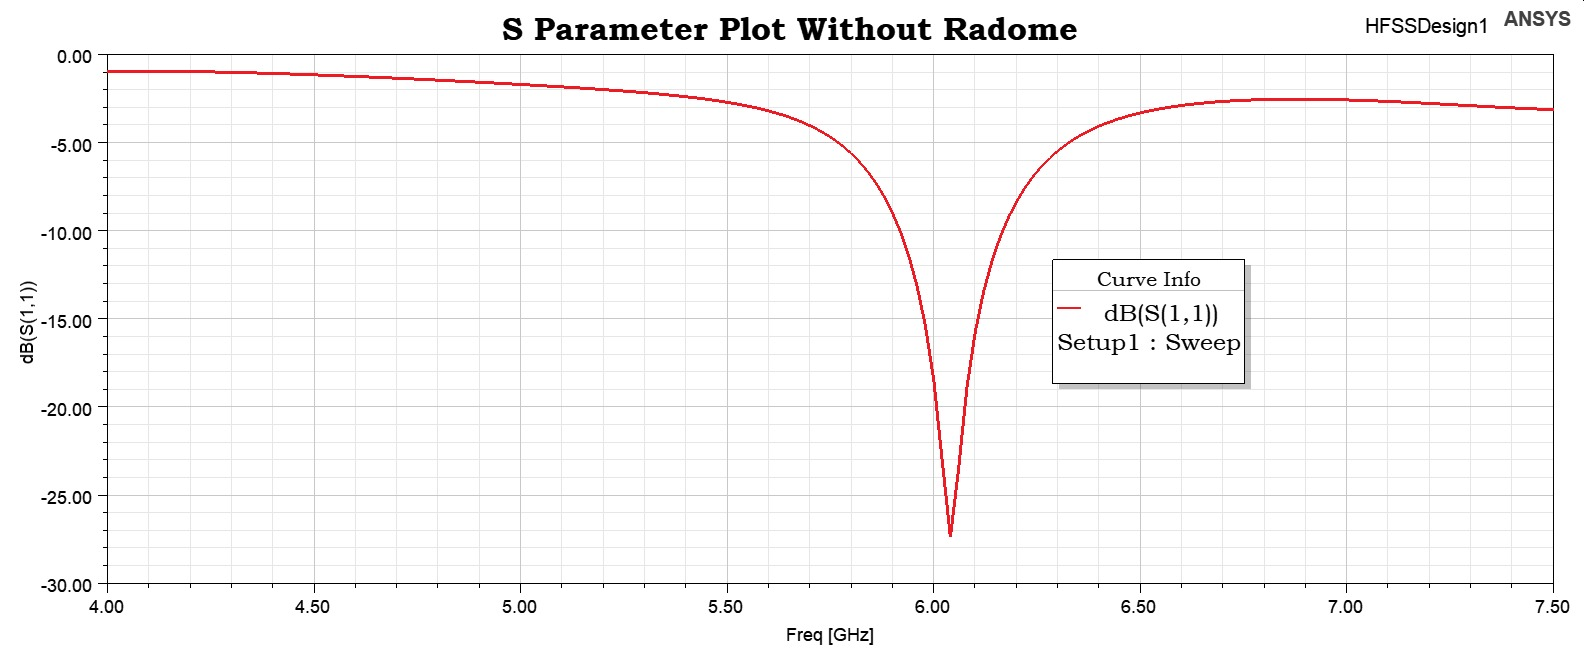
\includegraphics[width=1.0\textwidth]{figures/without_radome/s11.jpeg}
    \caption{Simulated S11 (return loss) of the patch antenna without radome.}
    \label{fig:res-without-s11}
\end{figure}

Figure~\ref{fig:res-without-s11} illustrates the return loss (S11) performance of the patch antenna in free space. The deep notch around the center frequency (approximately 6 GHz) indicates efficient impedance matching, as values below $-10$ dB suggest minimal reflection. The sharper and deeper the dip, the better the resonance quality.

\begin{figure}[H]
    \centering
    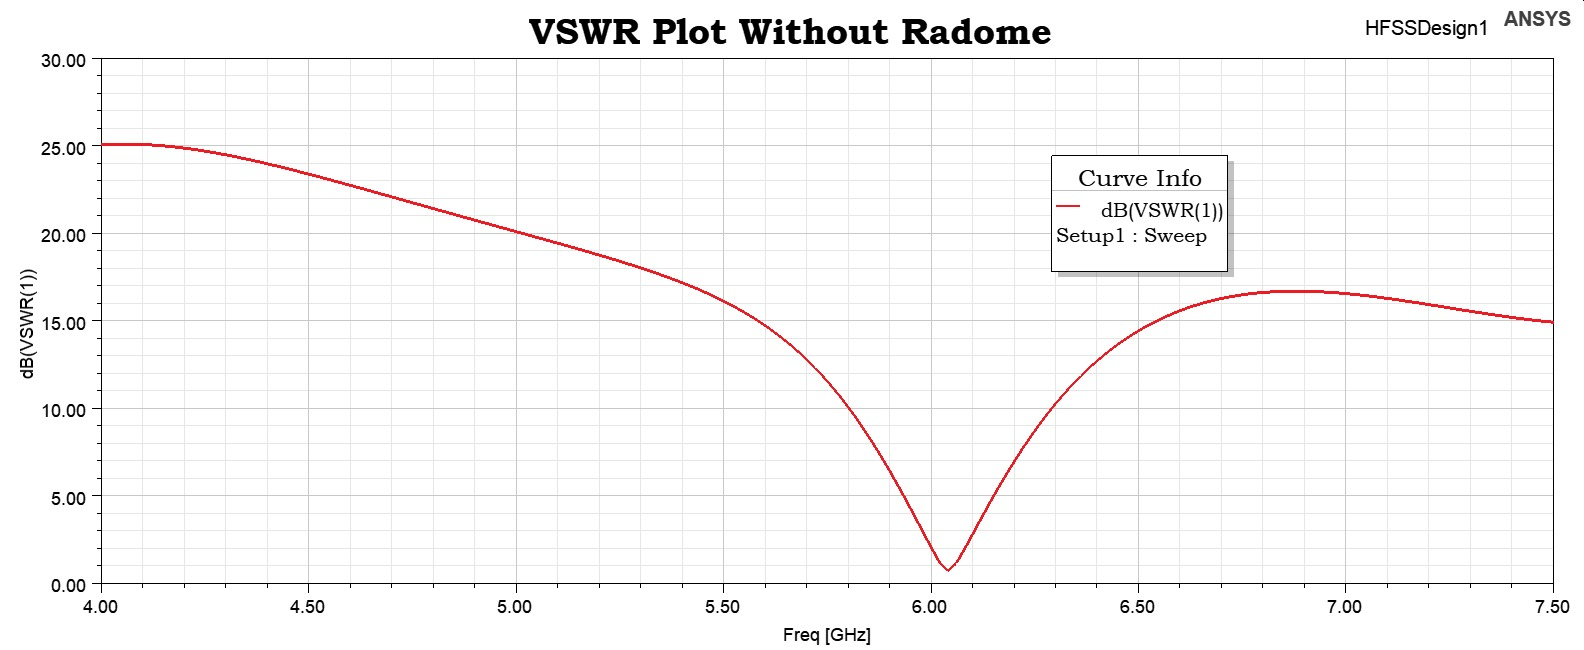
\includegraphics[width=1.0\textwidth]{figures/without_radome/VSWR.jpeg}
    \caption{Simulated VSWR of the patch antenna without radome.}
    \label{fig:res-without-vswr}
\end{figure}

The VSWR plot in Figure~\ref{fig:res-without-vswr} shows a corresponding dip near 6 GHz. A VSWR close to 1 indicates ideal matching, and values below 2 are generally acceptable. The shape and location of the curve match the S11 data, further validating the antenna's tuning.

\subsection{Gain Characteristics}

\begin{figure}[H]
    \centering
    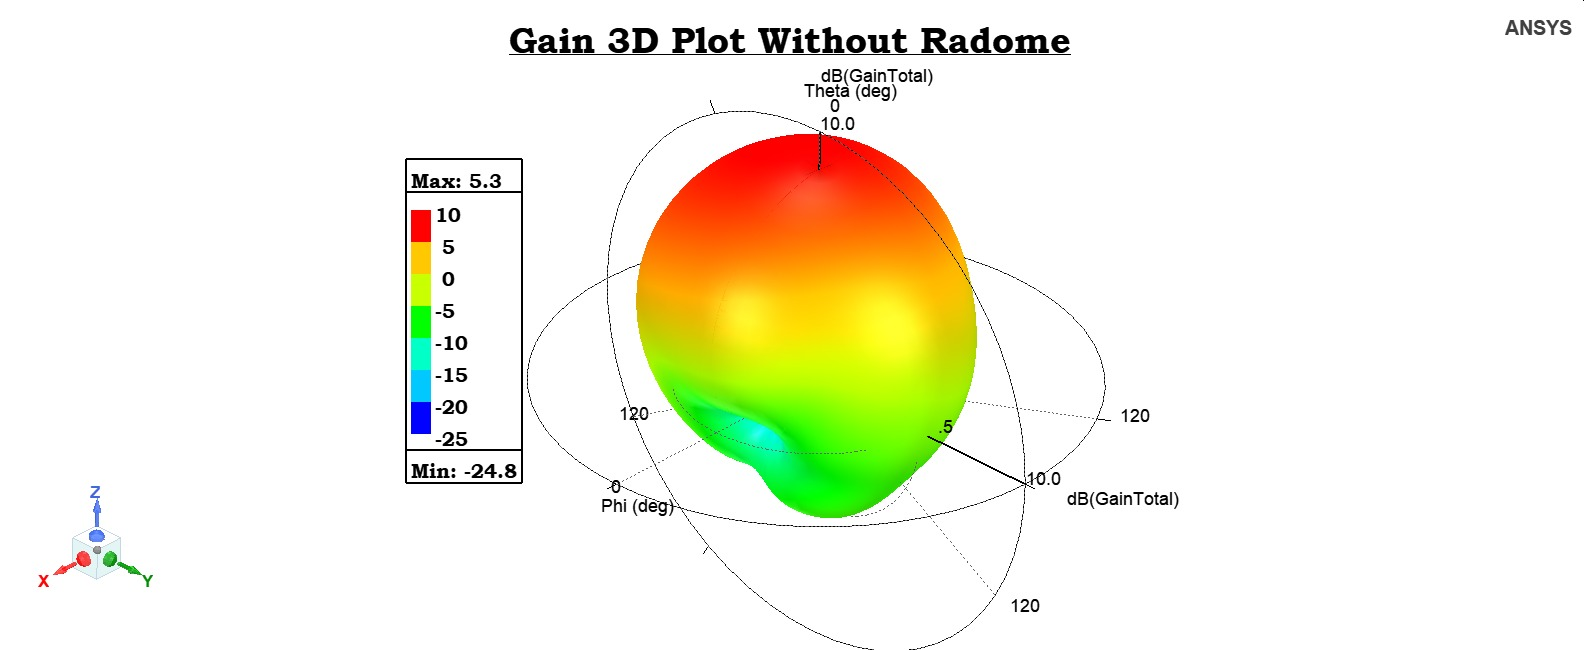
\includegraphics[width=1.0\textwidth]{figures/without_radome/gain plot.jpeg}
    \caption{Simulated gain of the patch antenna without radome.}
    \label{fig:res-without-gain}
\end{figure}

Figure~\ref{fig:res-without-gain} presents the frequency response of gain. The gain peaks near resonance and gradually falls off toward the band edges, a typical trend in patch antennas. This result reflects good radiation efficiency with a directional pattern. The gain level is suitable for point-to-point or sector-based wireless communication applications.

\begin{figure}[H]
    \centering
    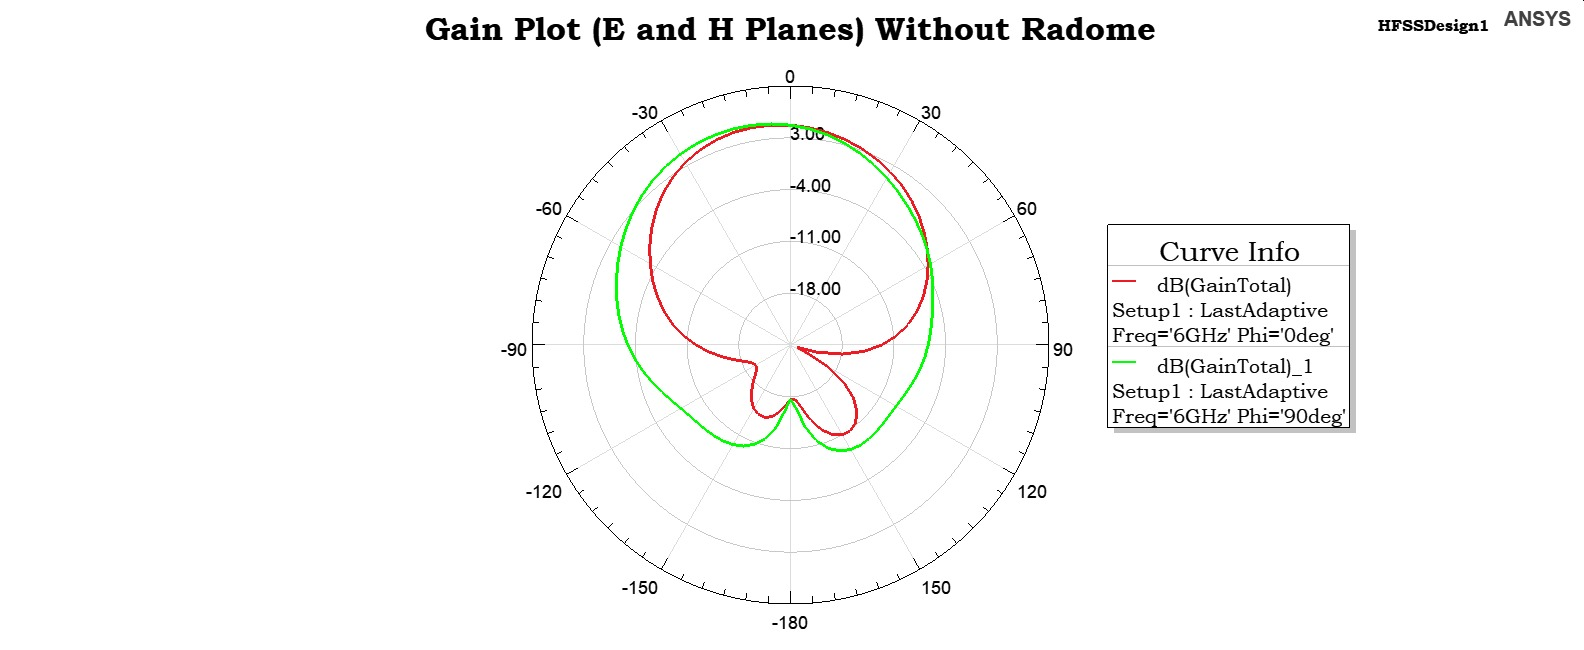
\includegraphics[width=1.0\textwidth]{figures/without_radome/Gain.jpeg}
    \caption{Gain pattern of the patch antenna without radome in both E-plane and H-plane.}
    \label{fig:res-gain-ehplane}
\end{figure}

Figure~\ref{fig:res-gain-ehplane} presents the 2D radiation patterns in the principal planes. The E-plane (elevation cut) shows the variation of gain with respect to vertical angle, while the H-plane (azimuthal cut) illustrates gain variation in the horizontal plane. The patterns confirm the directional behavior of the antenna and reveal its symmetry and front-to-back ratio. The close alignment of the main lobes in both planes suggests well-controlled beam shaping.

\subsection{Additional \texorpdfstring{$rE$}{rE} Overview}

\begin{figure}[H]
    \centering
    \includegraphics[width=1.0\textwidth]{figures/without_radome/co.jpeg}
    \caption{Co-polarization response of the patch antenna without radome.}
    \label{fig:res-co}
\end{figure}

\begin{figure}[H]
    \centering
    \includegraphics[width=1.0\textwidth]{figures/without_radome/cross.jpeg}
    \caption{Cross-polarization response of the patch antenna without radome.}
    \label{fig:res-cross}
\end{figure}

Figures~\ref{fig:res-co} and \ref{fig:res-cross} illustrate the co-polarization and cross-polarization responses of the patch antenna in the absence of a radome. The co-polarized field represents the desired polarization component aligned with the antenna's radiating axis, while the cross-polarized field indicates orthogonal components that are typically unwanted.

The co-polarization plot shows a strong, well-defined main lobe centered around the boresight, confirming that the antenna radiates efficiently in the intended polarization. In contrast, the cross-polarization level remains significantly lower across all angles, indicating minimal polarization leakage and strong polarization purity—an important factor in communication systems that rely on polarization isolation.

\begin{figure}[H]
    \centering
    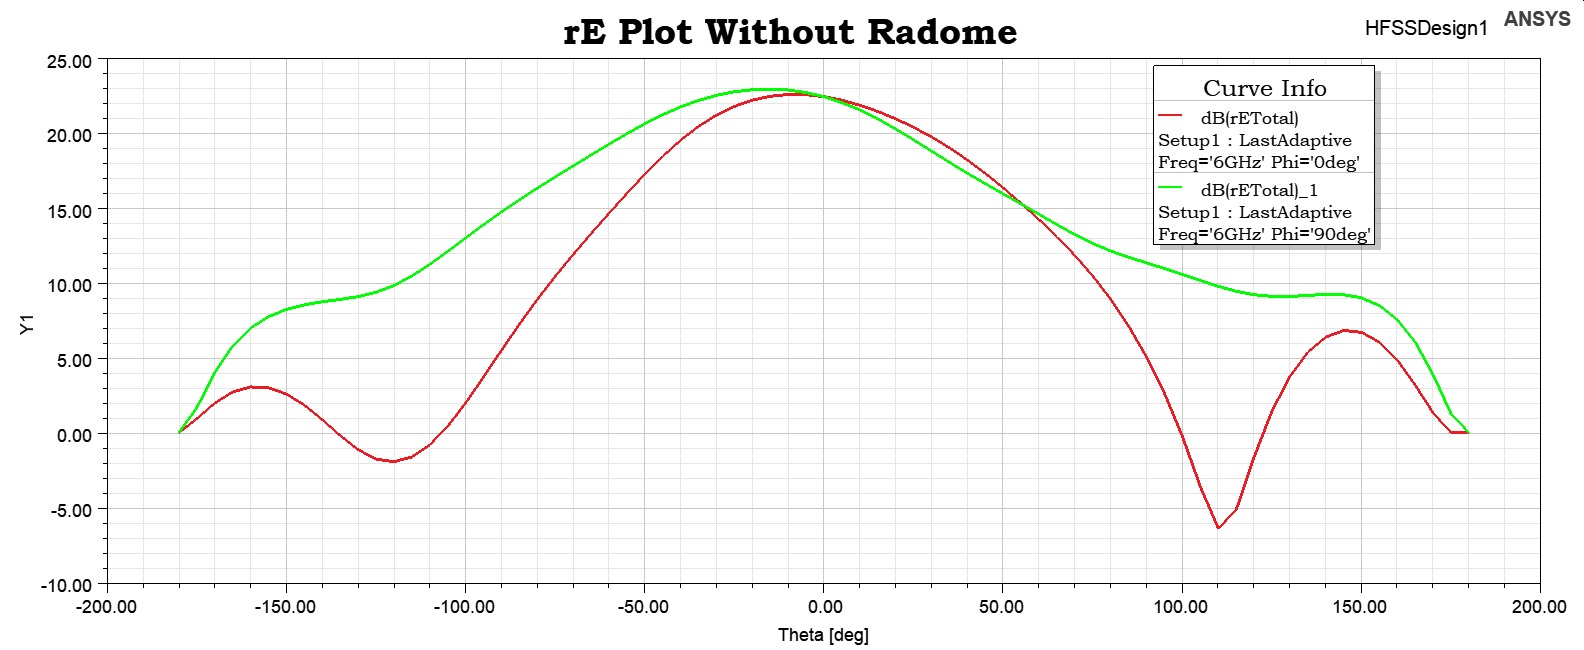
\includegraphics[width=1.0\textwidth]{figures/without_radome/rE.jpeg}
    \caption{General $rE$ field distribution without radome.}
    \label{fig:res-flat-re-overview}
\end{figure}

Figure~\ref{fig:res-flat-re-overview} shows the normalized electric field distribution ($rE$) in the far field. The pattern is symmetric and exhibits a broadside radiation characteristic, with energy concentrated normal to the patch surface. The absence of asymmetries or spurious sidelobes further confirms that the antenna operates as intended without distortions caused by external structures such as radomes.

\subsection{Parametric Sweep of Inset Feed}

\begin{figure}[H]
    \centering
    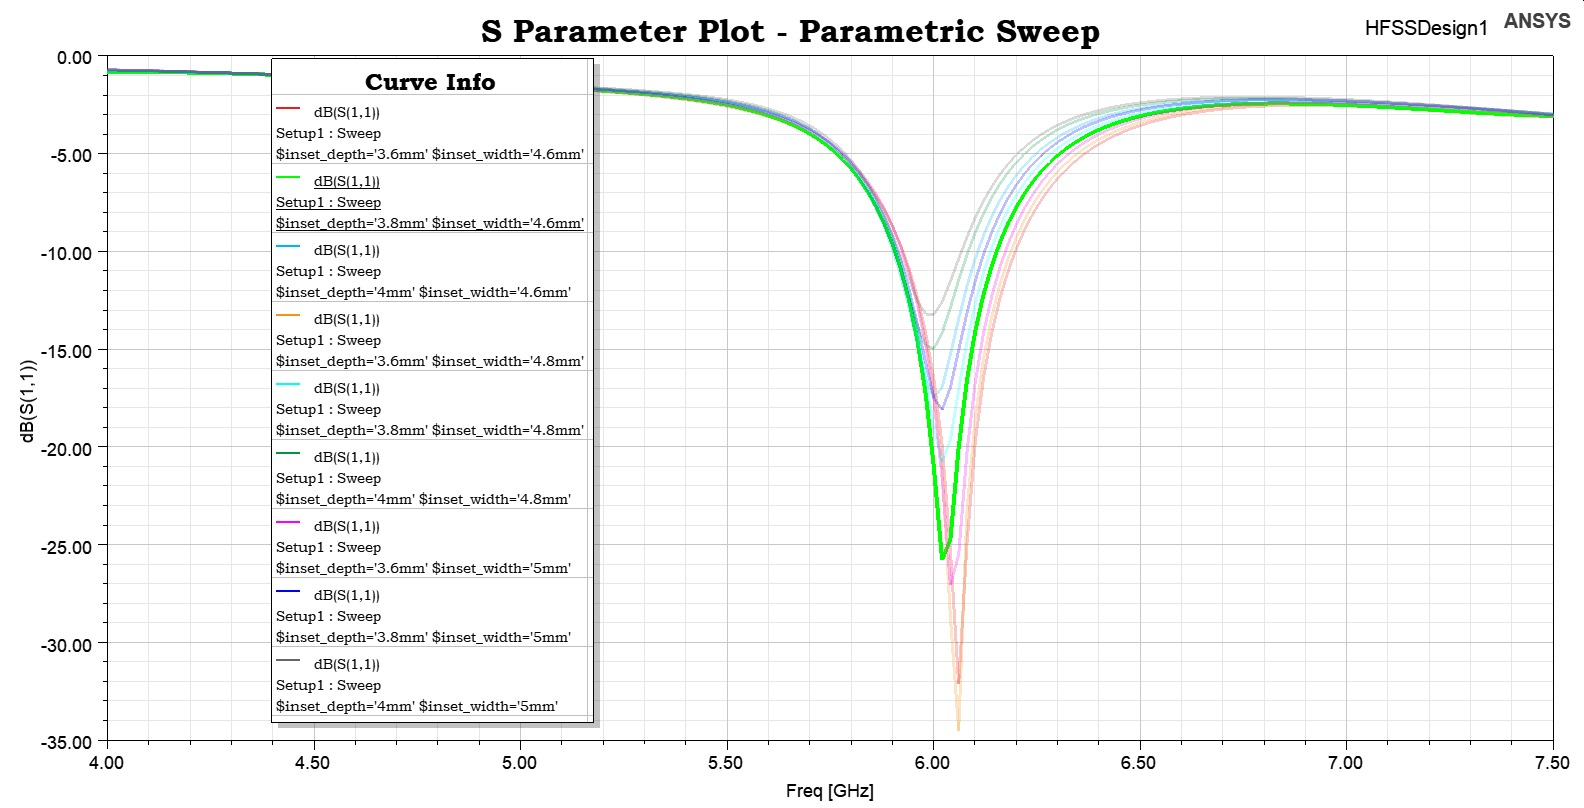
\includegraphics[width=1.0\textwidth]{figures/parametric_sweep/best parameter.jpeg}
    \caption{Identified optimal inset feed parameters from the parametric sweep.}
    \label{fig:res-param-best}
\end{figure}

Figure~\ref{fig:res-param-best} summarizes the optimal inset feed location and width for achieving best impedance match. Proper tuning of these parameters is critical for maximum power transfer and is reflected in a lower S11 and better VSWR.

\begin{figure}[H]
    \centering
    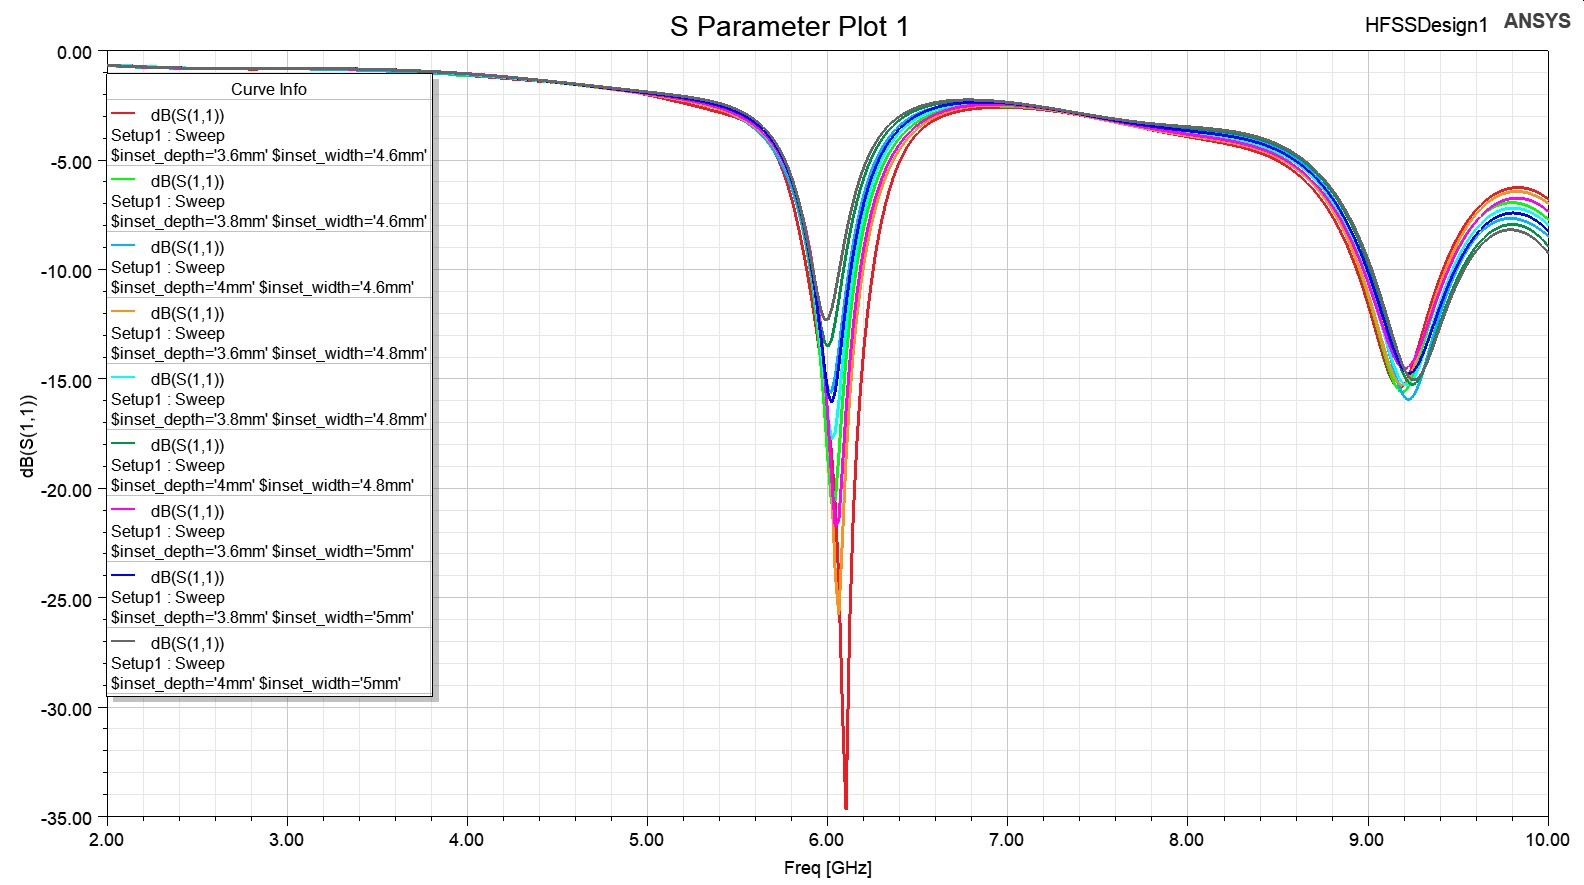
\includegraphics[width=1.0\textwidth]{figures/parametric_sweep/parametric analysis.jpeg}
    \caption{General overview of the parametric analysis for feed inset optimization.}
    \label{fig:res-param-analysis}
\end{figure}

Figure~\ref{fig:res-param-analysis} demonstrates the effect of varying feed positions on return loss. The ideal combination is the one that yields the deepest notch around the target frequency. This iterative approach provides insights into the physical sensitivity of the antenna to feed location.

\noindent
Note: The same feed dimensions will be reused for radome studies.

% -------------------------------------------------------------------

\section{Performance with Flat Radome}

\subsection{Parametric Sweep of Inter-Radome Distance}

\begin{figure}[H]
    \centering
    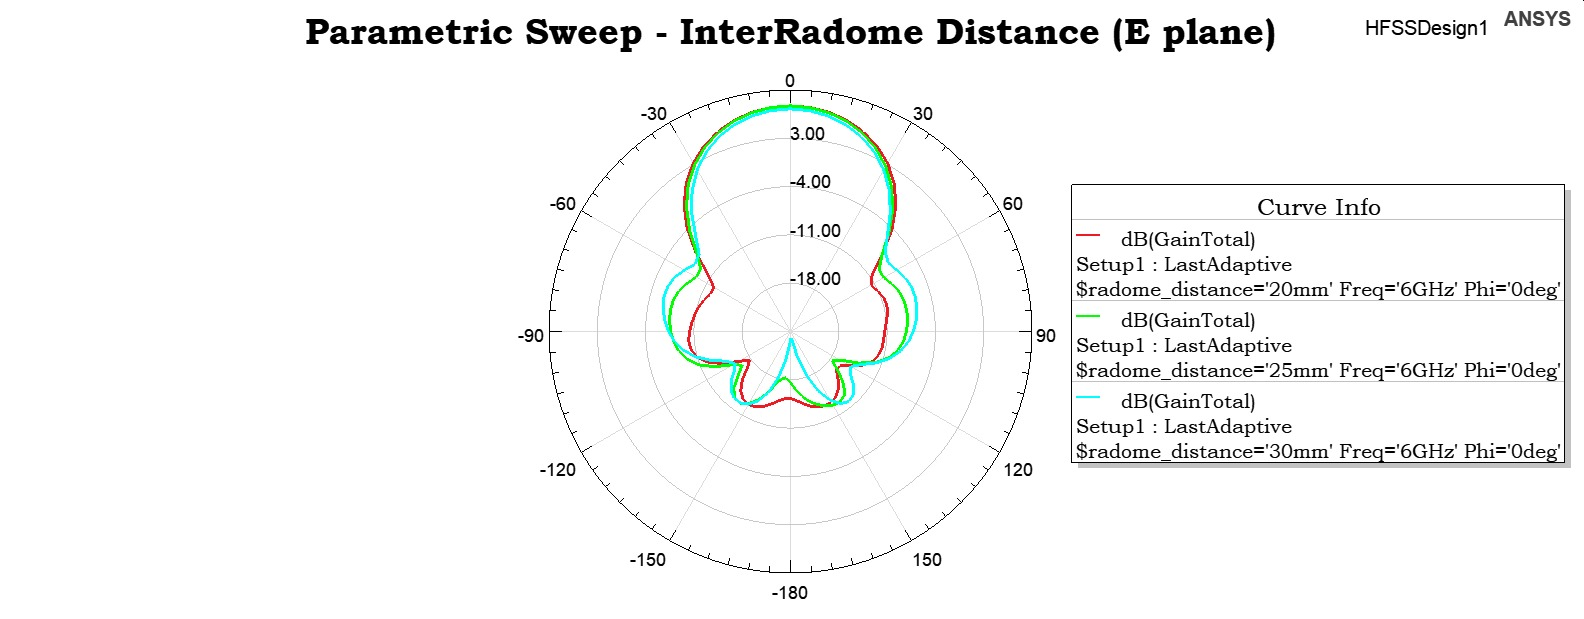
\includegraphics[width=1.0\textwidth]{figures/parametric_sweep/Radome distance (E plane).jpeg}
    \caption{Gain variation in the E-plane for different inter-radome (airgap) distances.}
    \label{fig:res-gap-gain-eplane}
\end{figure}

\begin{figure}[H]
    \centering
    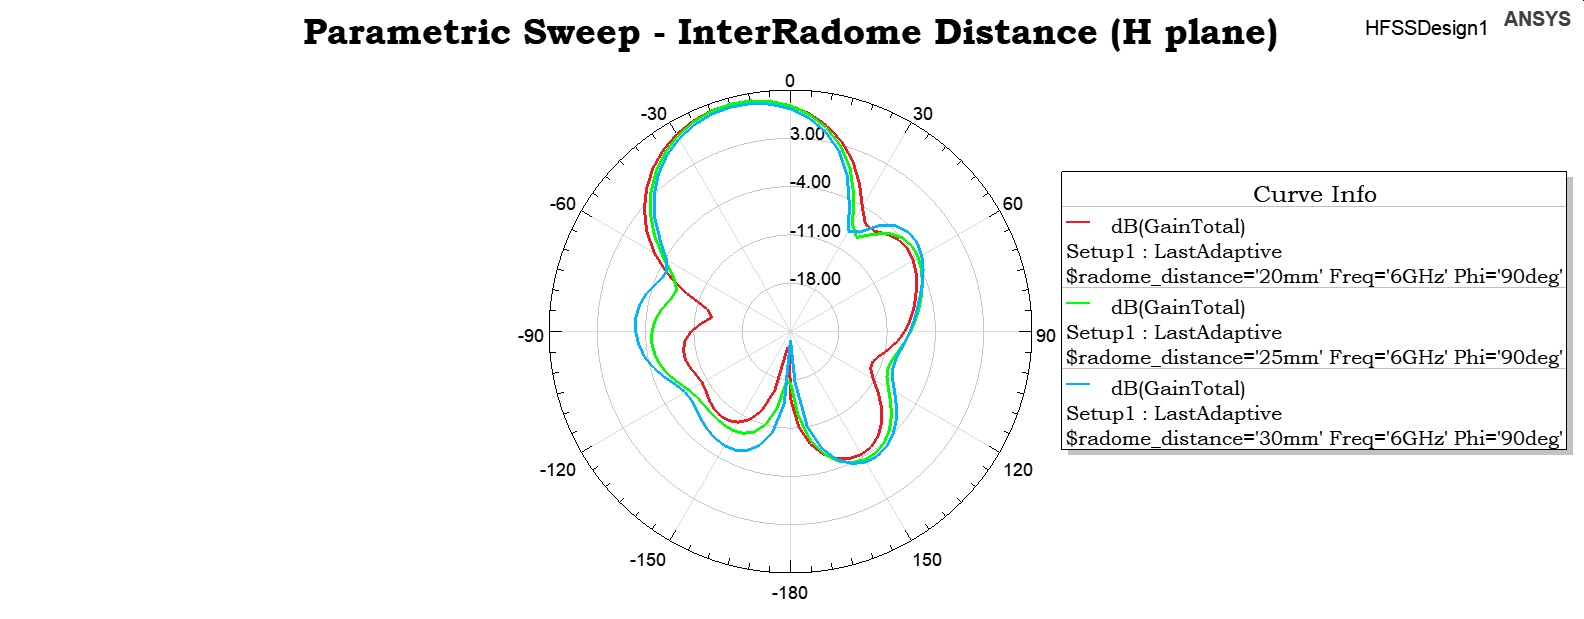
\includegraphics[width=1.0\textwidth]{figures/parametric_sweep/radome distance (H plane).jpeg}
    \caption{Gain variation in the H-plane for different inter-radome (airgap) distances.}
    \label{fig:res-gap-gain-hplane}
\end{figure}

Figures~\ref{fig:res-gap-gain-eplane} and \ref{fig:res-gap-gain-hplane} show how the gain pattern evolves in the E-plane and H-plane respectively as the distance between the antenna and the radome changes. Both plots highlight the existence of an optimal separation where gain is maximized due to constructive field interaction.

Deviating from this optimal point leads to degraded gain, caused by near-field phase mismatch and partial destructive interference. This reinforces the importance of careful mechanical design and spacing in practical antenna–radome integration.

\subsection{Gain Characteristics with Radome}

\begin{figure}[H]
    \centering
    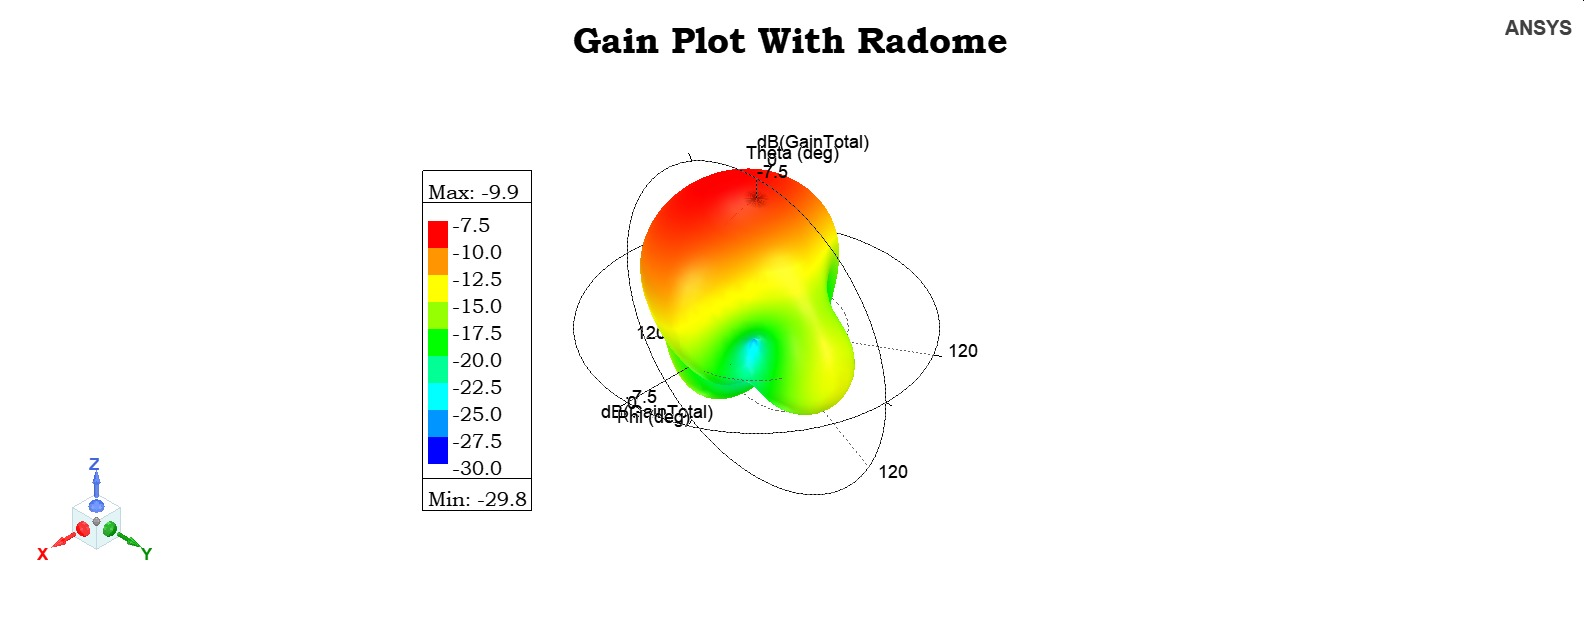
\includegraphics[width=1.0\textwidth]{figures/with_radome/gain plot.jpeg}
    \caption{Simulated gain of the patch antenna with flat radome.}
    \label{fig:res-with-gain-radome}
\end{figure}

Figure~\ref{fig:res-with-gain-radome} shows the gain response of the patch antenna when enclosed within a flat radome. While the overall shape of the curve remains similar to the no-radome case, a slight reduction in peak gain is observed, particularly near the resonant frequency. This reduction is attributed to dielectric loading and partial reflection losses introduced by the radome material. Despite this, the antenna still maintains a directional radiation pattern with adequate gain for practical deployment, indicating that the radome's impact on gain is minimal.

\subsection{Return Loss and VSWR}

\begin{figure}[H]
    \centering
    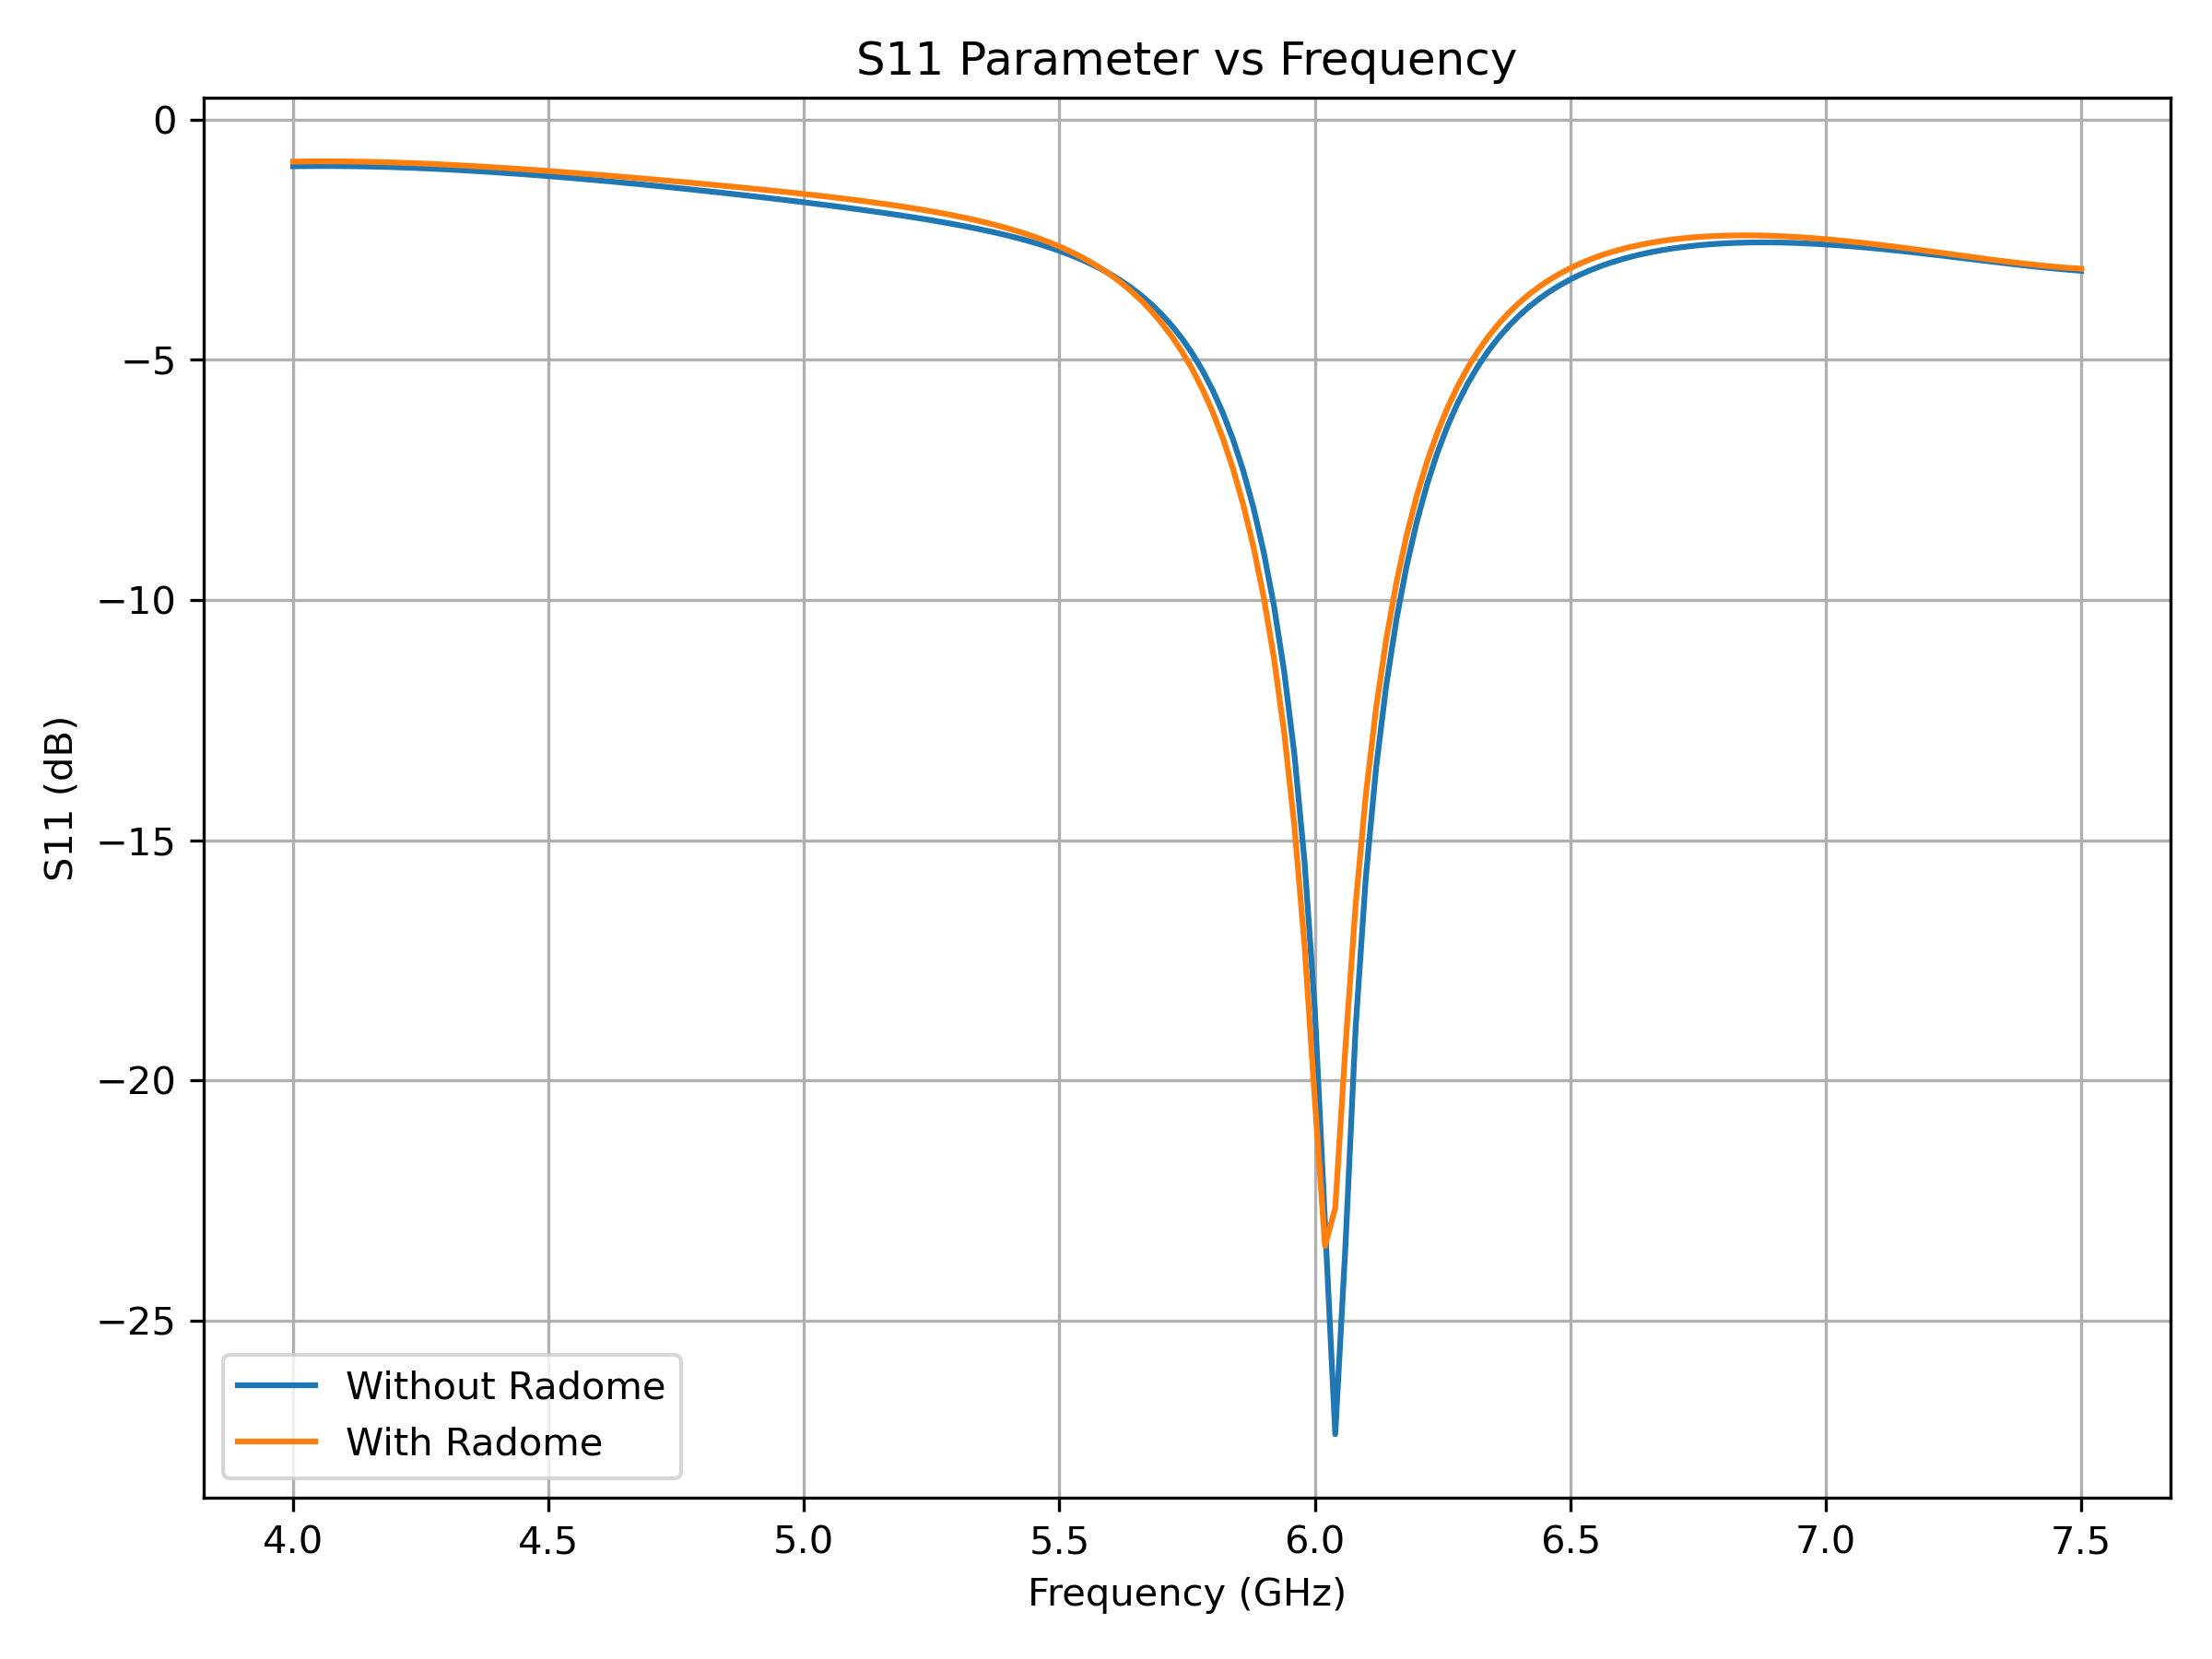
\includegraphics[width=1.0\textwidth]{figures/comparison_flat_radome/s11.png}
    \caption{Simulated S11 of the patch antenna with flat radome.}
    \label{fig:res-flat-s11}
\end{figure}

Figure~\ref{fig:res-flat-s11} depicts a noticeable shift in the return loss curve due to the introduction of the PMMA radome. The frequency shift indicates a slight detuning effect caused by the dielectric loading. The dip is slightly shallower, suggesting marginal impedance mismatch introduced by the radome material.

\begin{figure}[H]
    \centering
    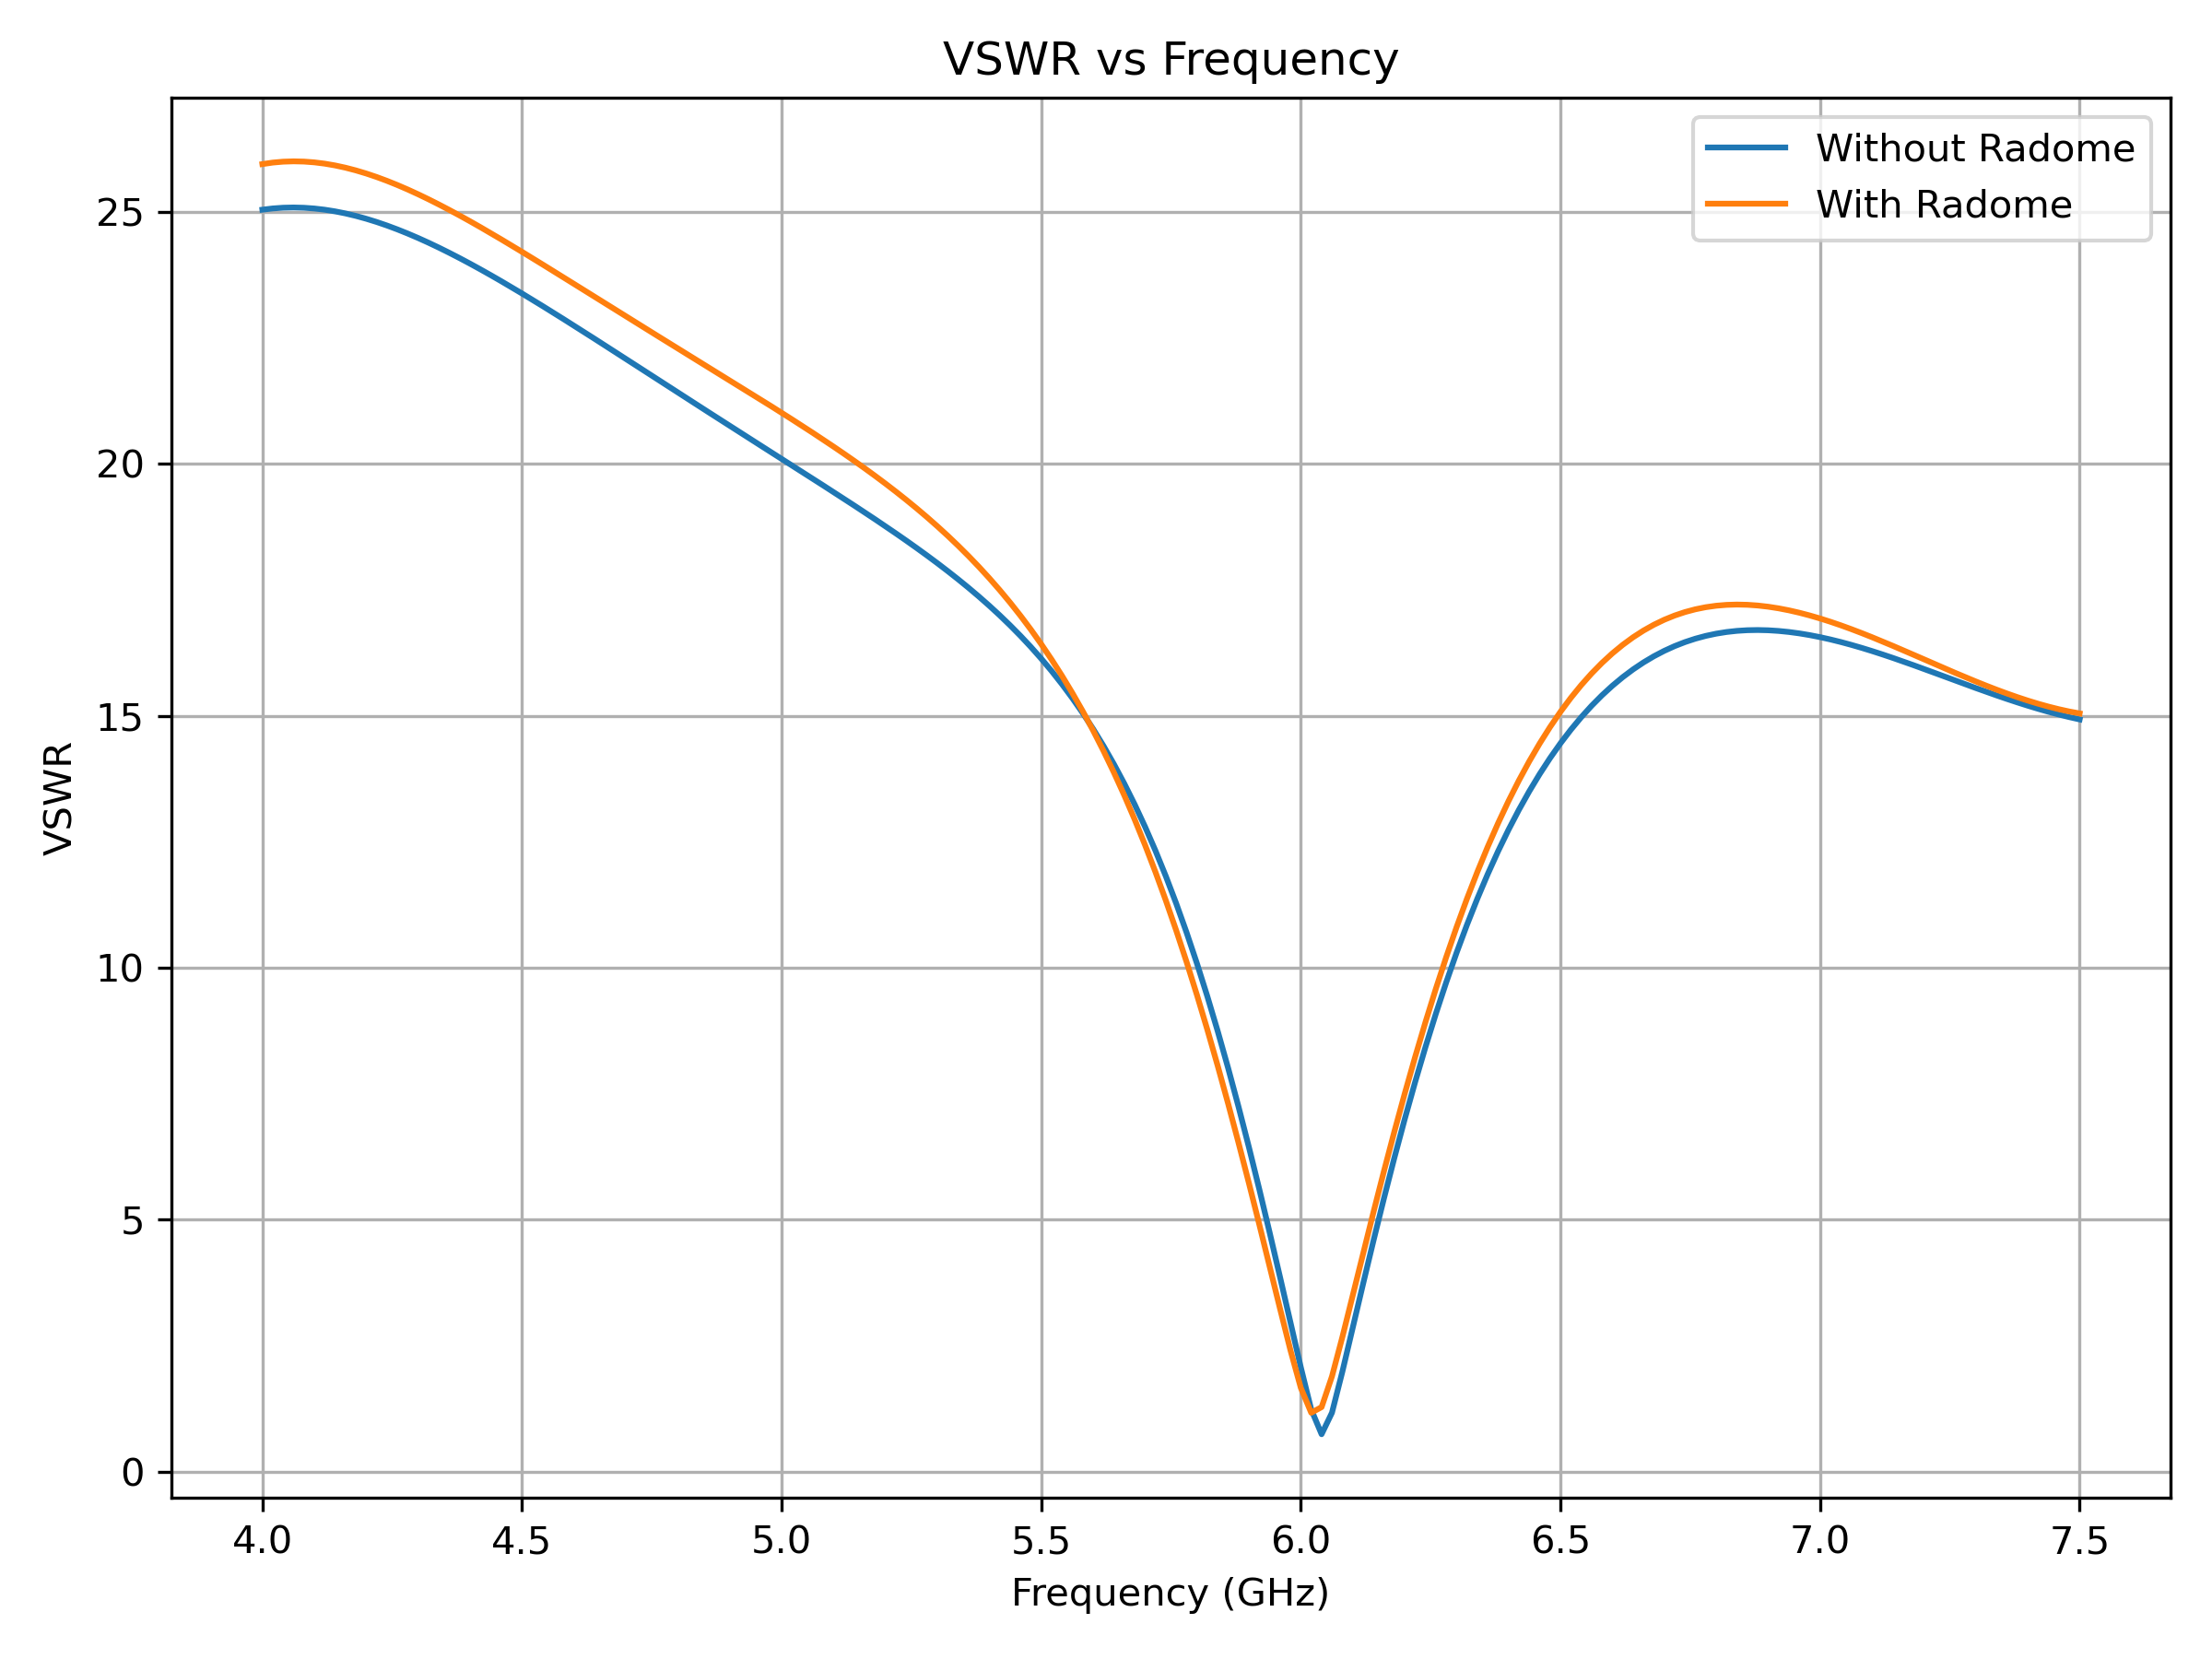
\includegraphics[width=1.0\textwidth]{figures/comparison_flat_radome/vswr.png}
    \caption{Simulated VSWR of the patch antenna with flat radome.}
    \label{fig:res-flat-vswr}
\end{figure}

In Figure~\ref{fig:res-flat-vswr}, the VSWR is slightly higher than the baseline case, reinforcing the return loss trend. Although still under 2, indicating acceptable performance, the result confirms that the radome introduces a small impedance mismatch.

\subsection{Gain across Frequencies (E-Plane)}

The E-plane gain patterns (phi=0°) show the antenna's performance with and without a radome at various frequencies.

\begin{figure}[H]
\centering
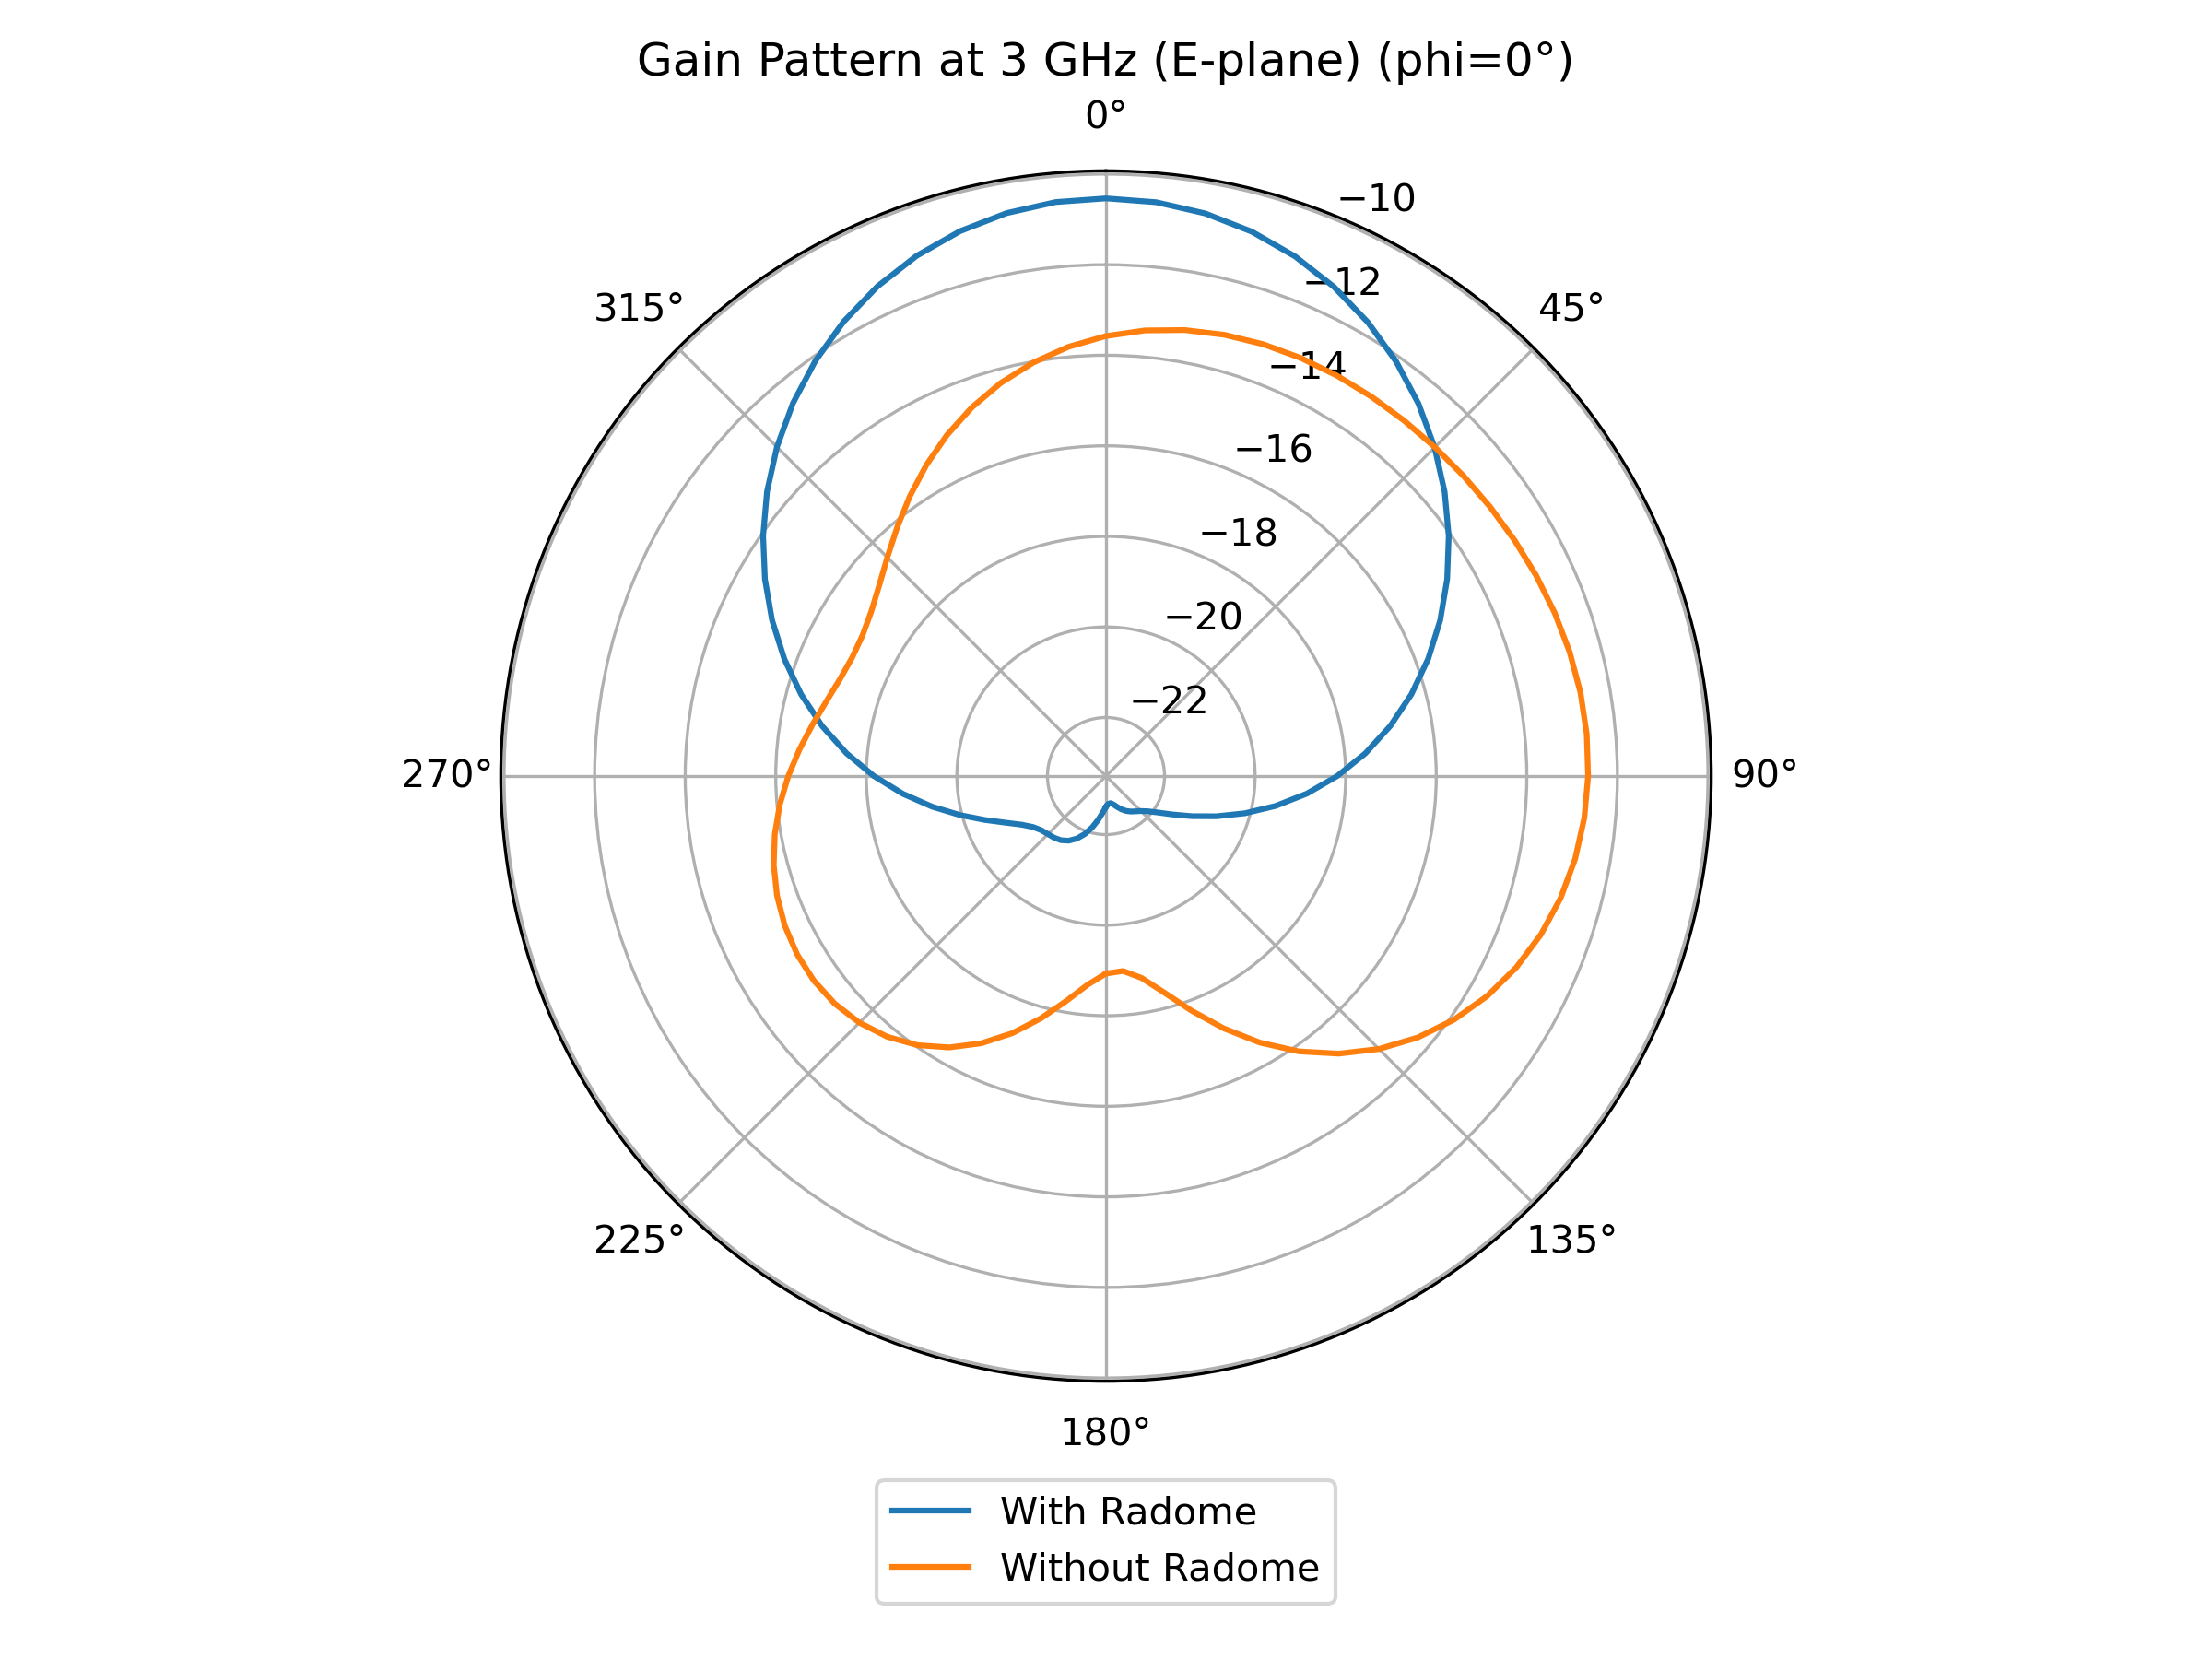
\includegraphics[width=1.0\textwidth]{figures/comparison_flat_radome/gainE_3_GHz.png}
\caption{Simulated gain of the patch antenna with flat radome at 3,GHz.}
\label{fig:res-flat-gainE3}
\end{figure}

Figure~\ref{fig:res-flat-gainE3} illustrates the radiation performance at the lower edge of the band (3 GHz) in the E-plane. Here, the gain of the antenna with the flat radome (blue line) is noticeably reduced compared to the free-space performance (orange line), particularly in the main lobe. The maximum gain without the radome is around -12 dB, while with the radome, it increases to approximately -10 dB. This suggests increased reflection and possible absorption by the radome at this off-resonant frequency, leading to a degradation in performance.

\begin{figure}[H]
\centering
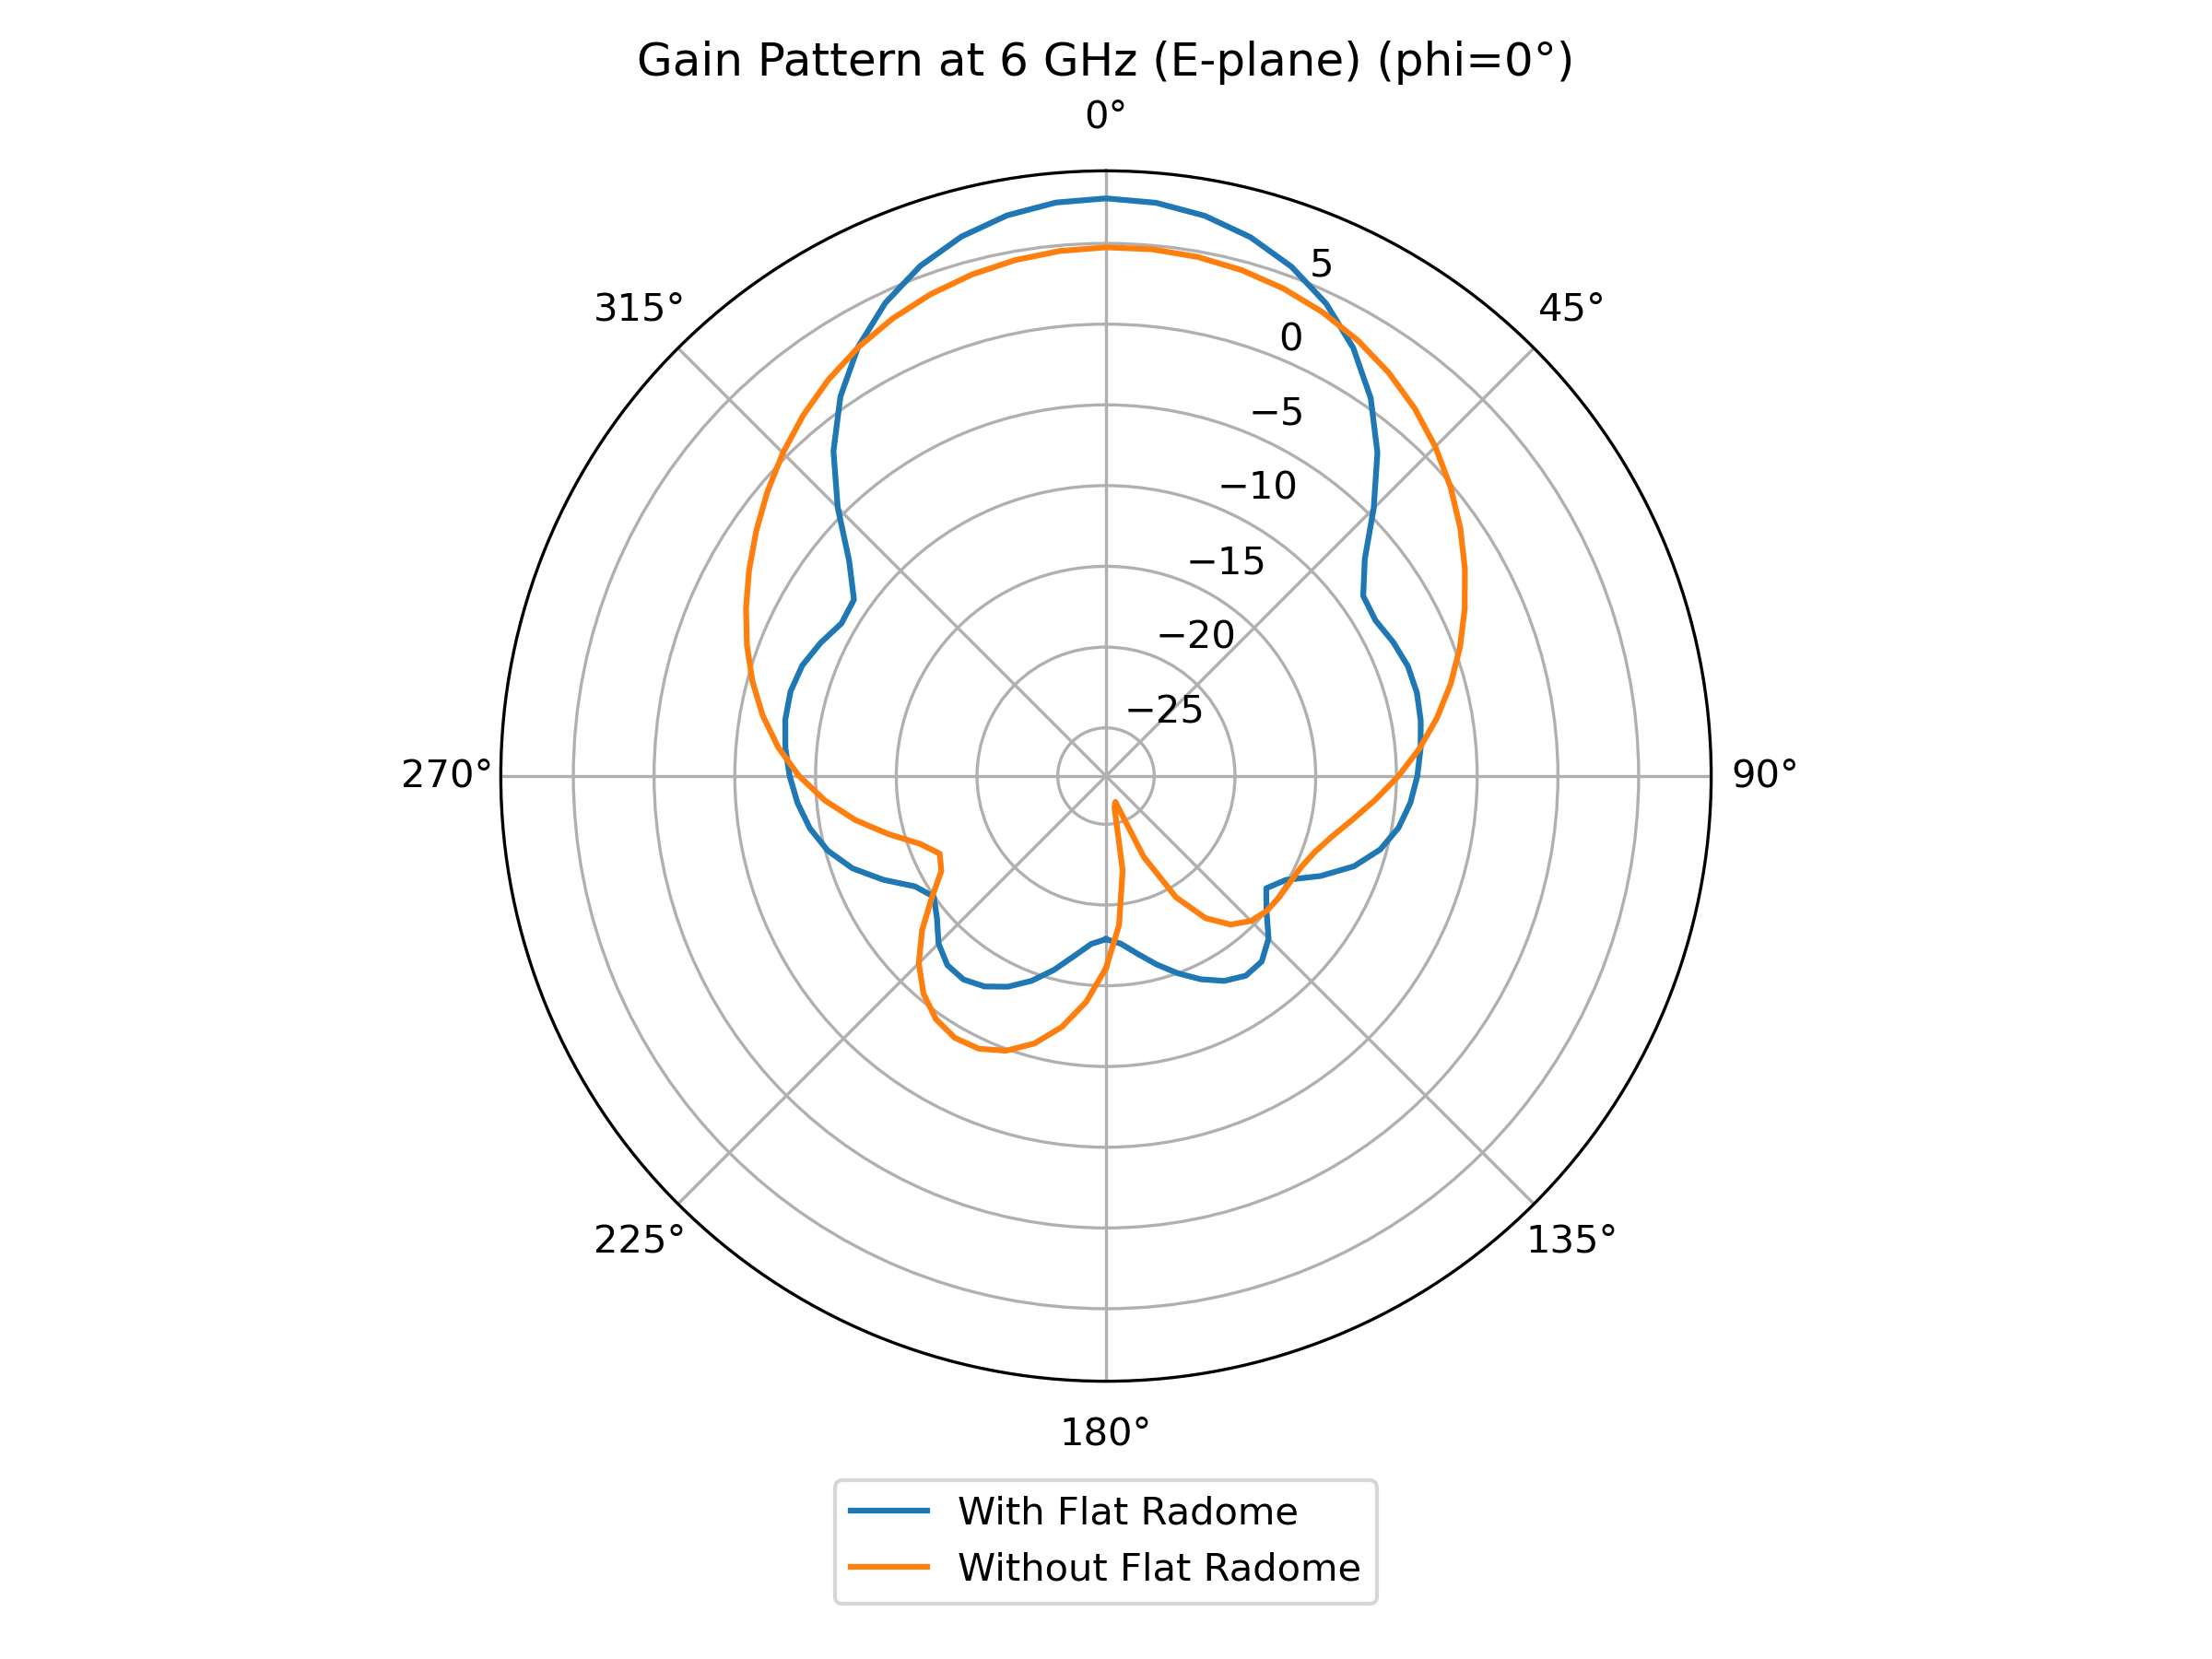
\includegraphics[width=1.0\textwidth]{figures/comparison_flat_radome/gainE_6_GHz.png}
\caption{Simulated gain of the patch antenna with flat radome at 6,GHz.}
\label{fig:res-flat-gainE6}
\end{figure}

At 6 GHz (Figure~\ref{fig:res-flat-gainE6}), which is closer to the antenna's presumed resonance frequency, the gain remains strong and closely matches the free-space case. The peak gain for both "With Radome" (blue line) and "Without Radome" (orange line) is approximately 5 dB. This indicates that the radome design is largely transparent and introduces minimal impact on the antenna's performance near its operating band center.

\begin{figure}[H]
\centering
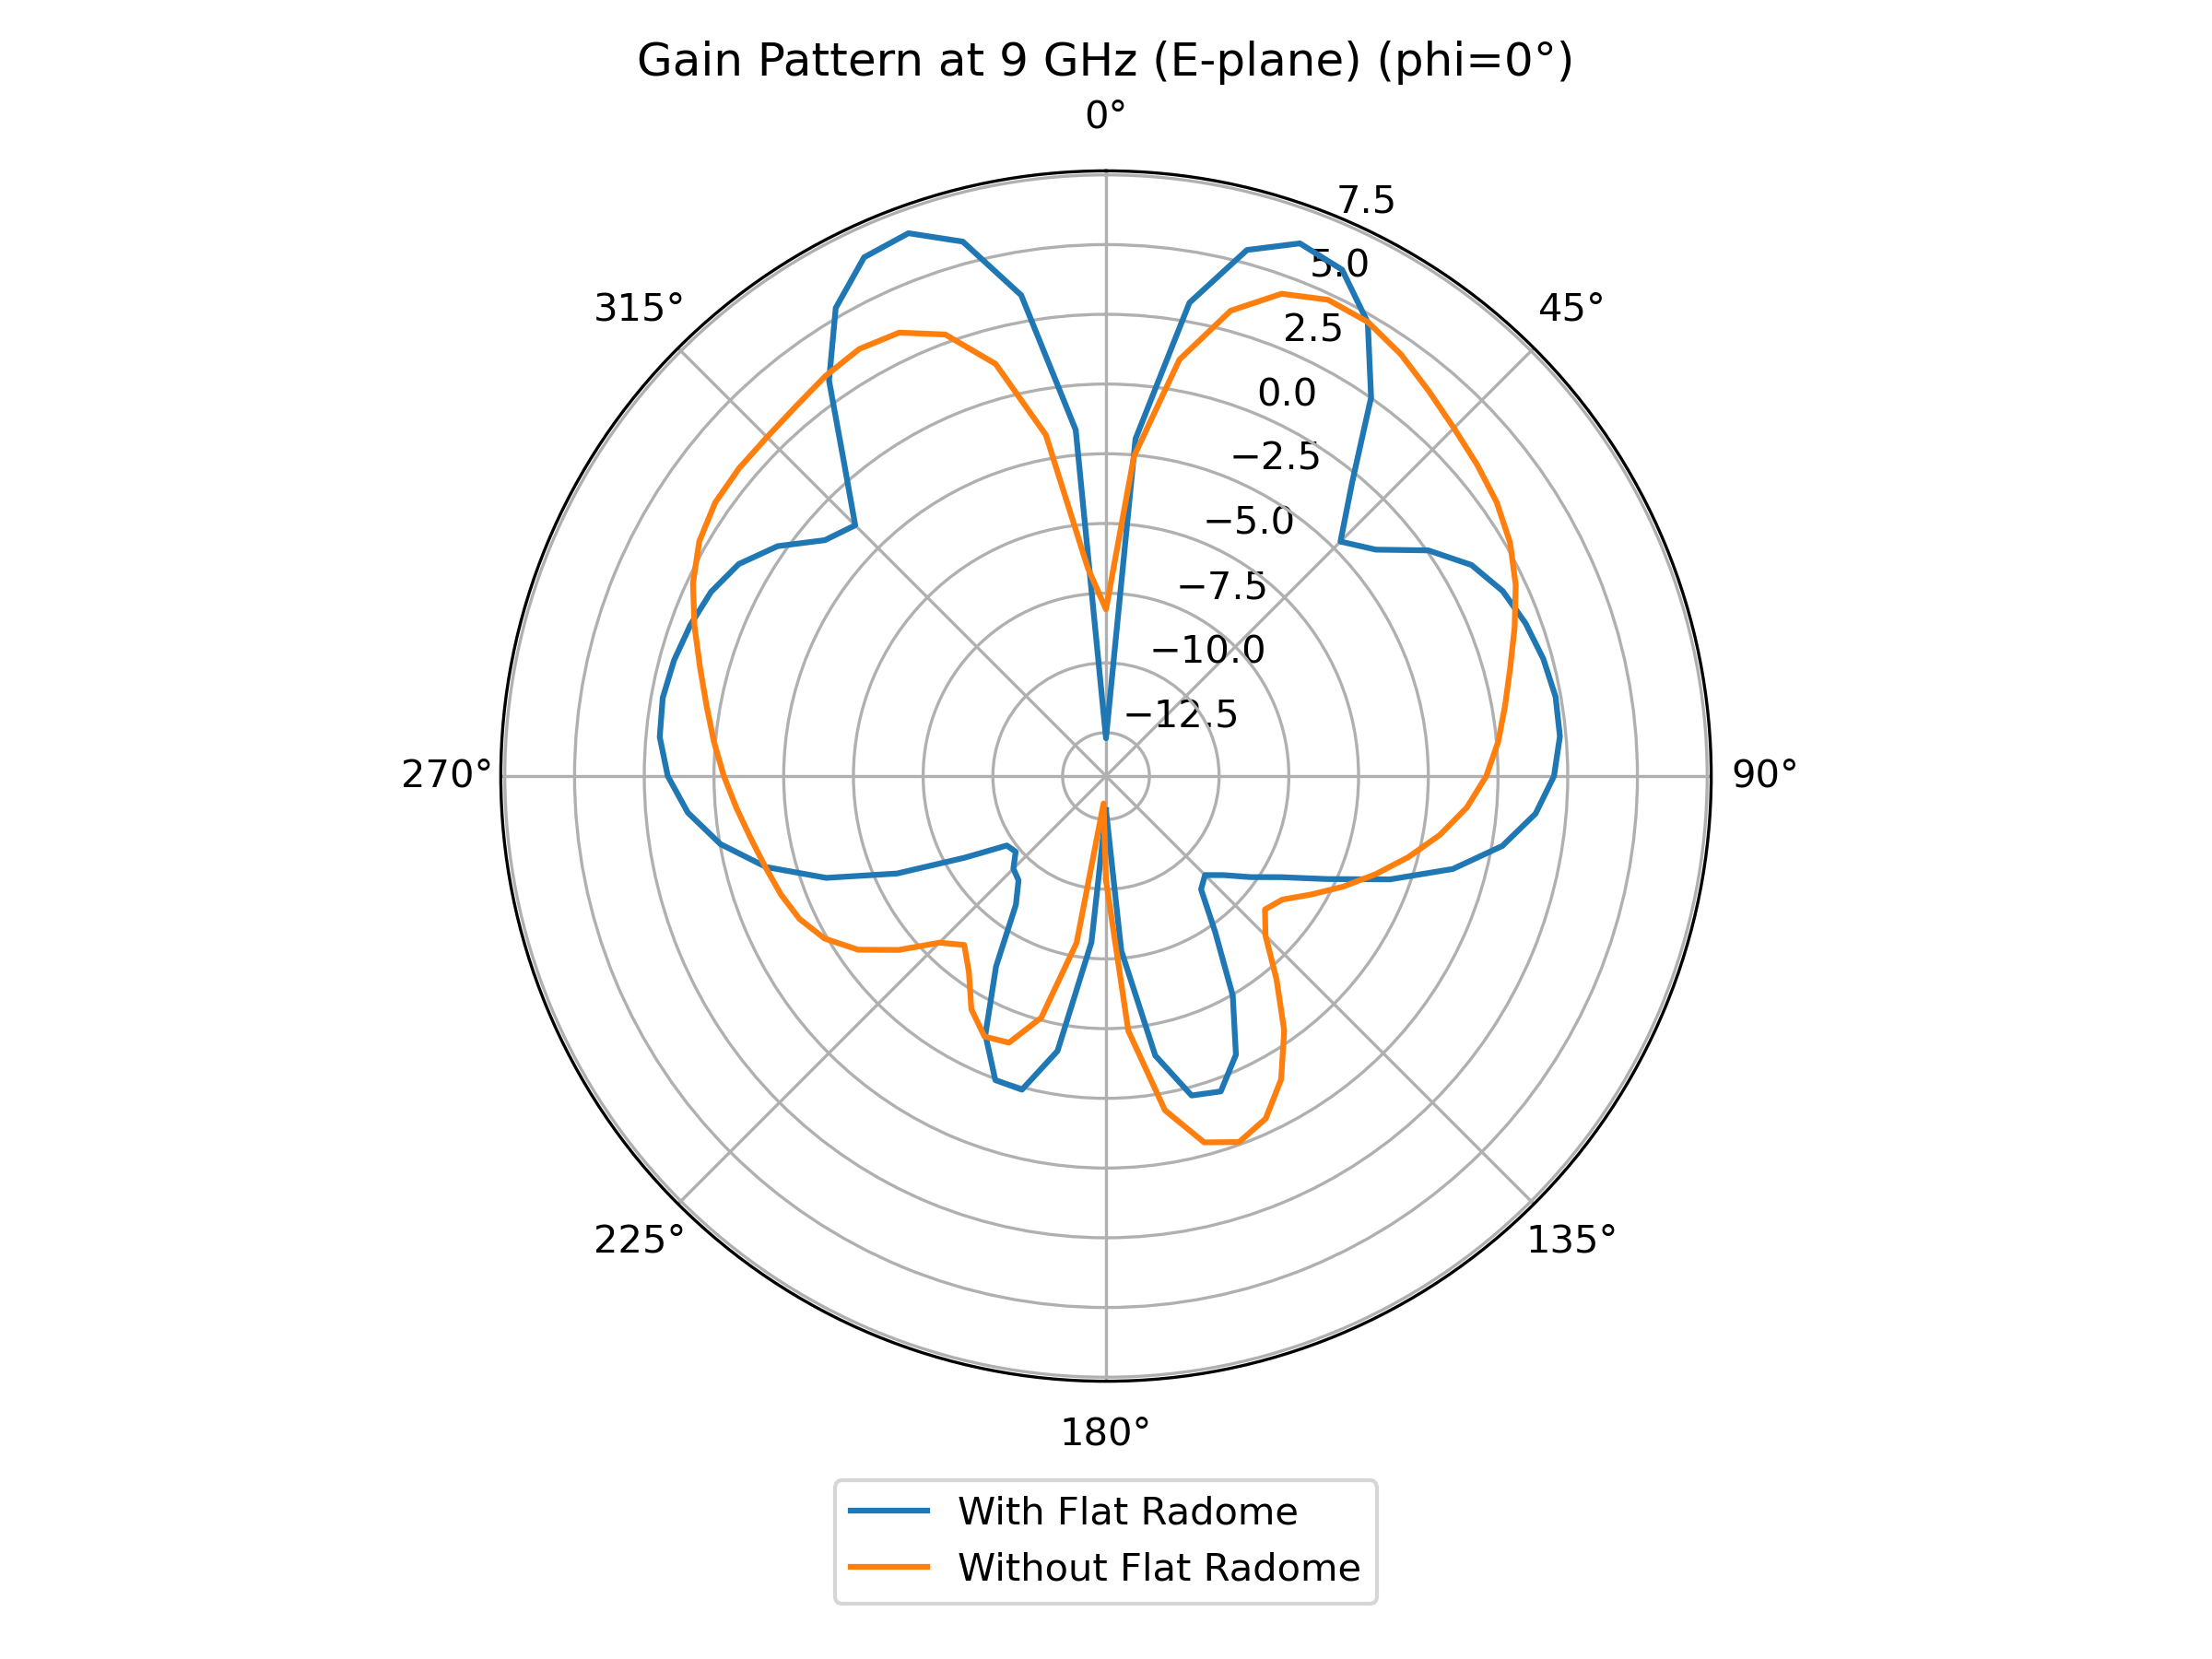
\includegraphics[width=1.0\textwidth]{figures/comparison_flat_radome/gainE_9_GHz.png}
\caption{Simulated gain of the patch antenna with flat radome at 9,GHz.}
\label{fig:res-flat-gainE9}
\end{figure}

Figure~\ref{fig:res-flat-gainE9} shows degradation in gain at the higher frequency end (9 GHz) in the E-plane. The maximum gain with the radome (blue line) is around 5 dB, whereas without the radome (orange line) it is closer to 2.5 dB. The radome causes a increase in the peak gain and also appears to slightly alter the shape of the main lobe, potentially introducing increased side lobe levels at this off-resonant frequency.

\subsection{Gain across Frequencies (H-Plane)}

The H-plane gain patterns (phi=90°) provide insight into the antenna's performance with and without a radome.

\begin{figure}[H]
\centering
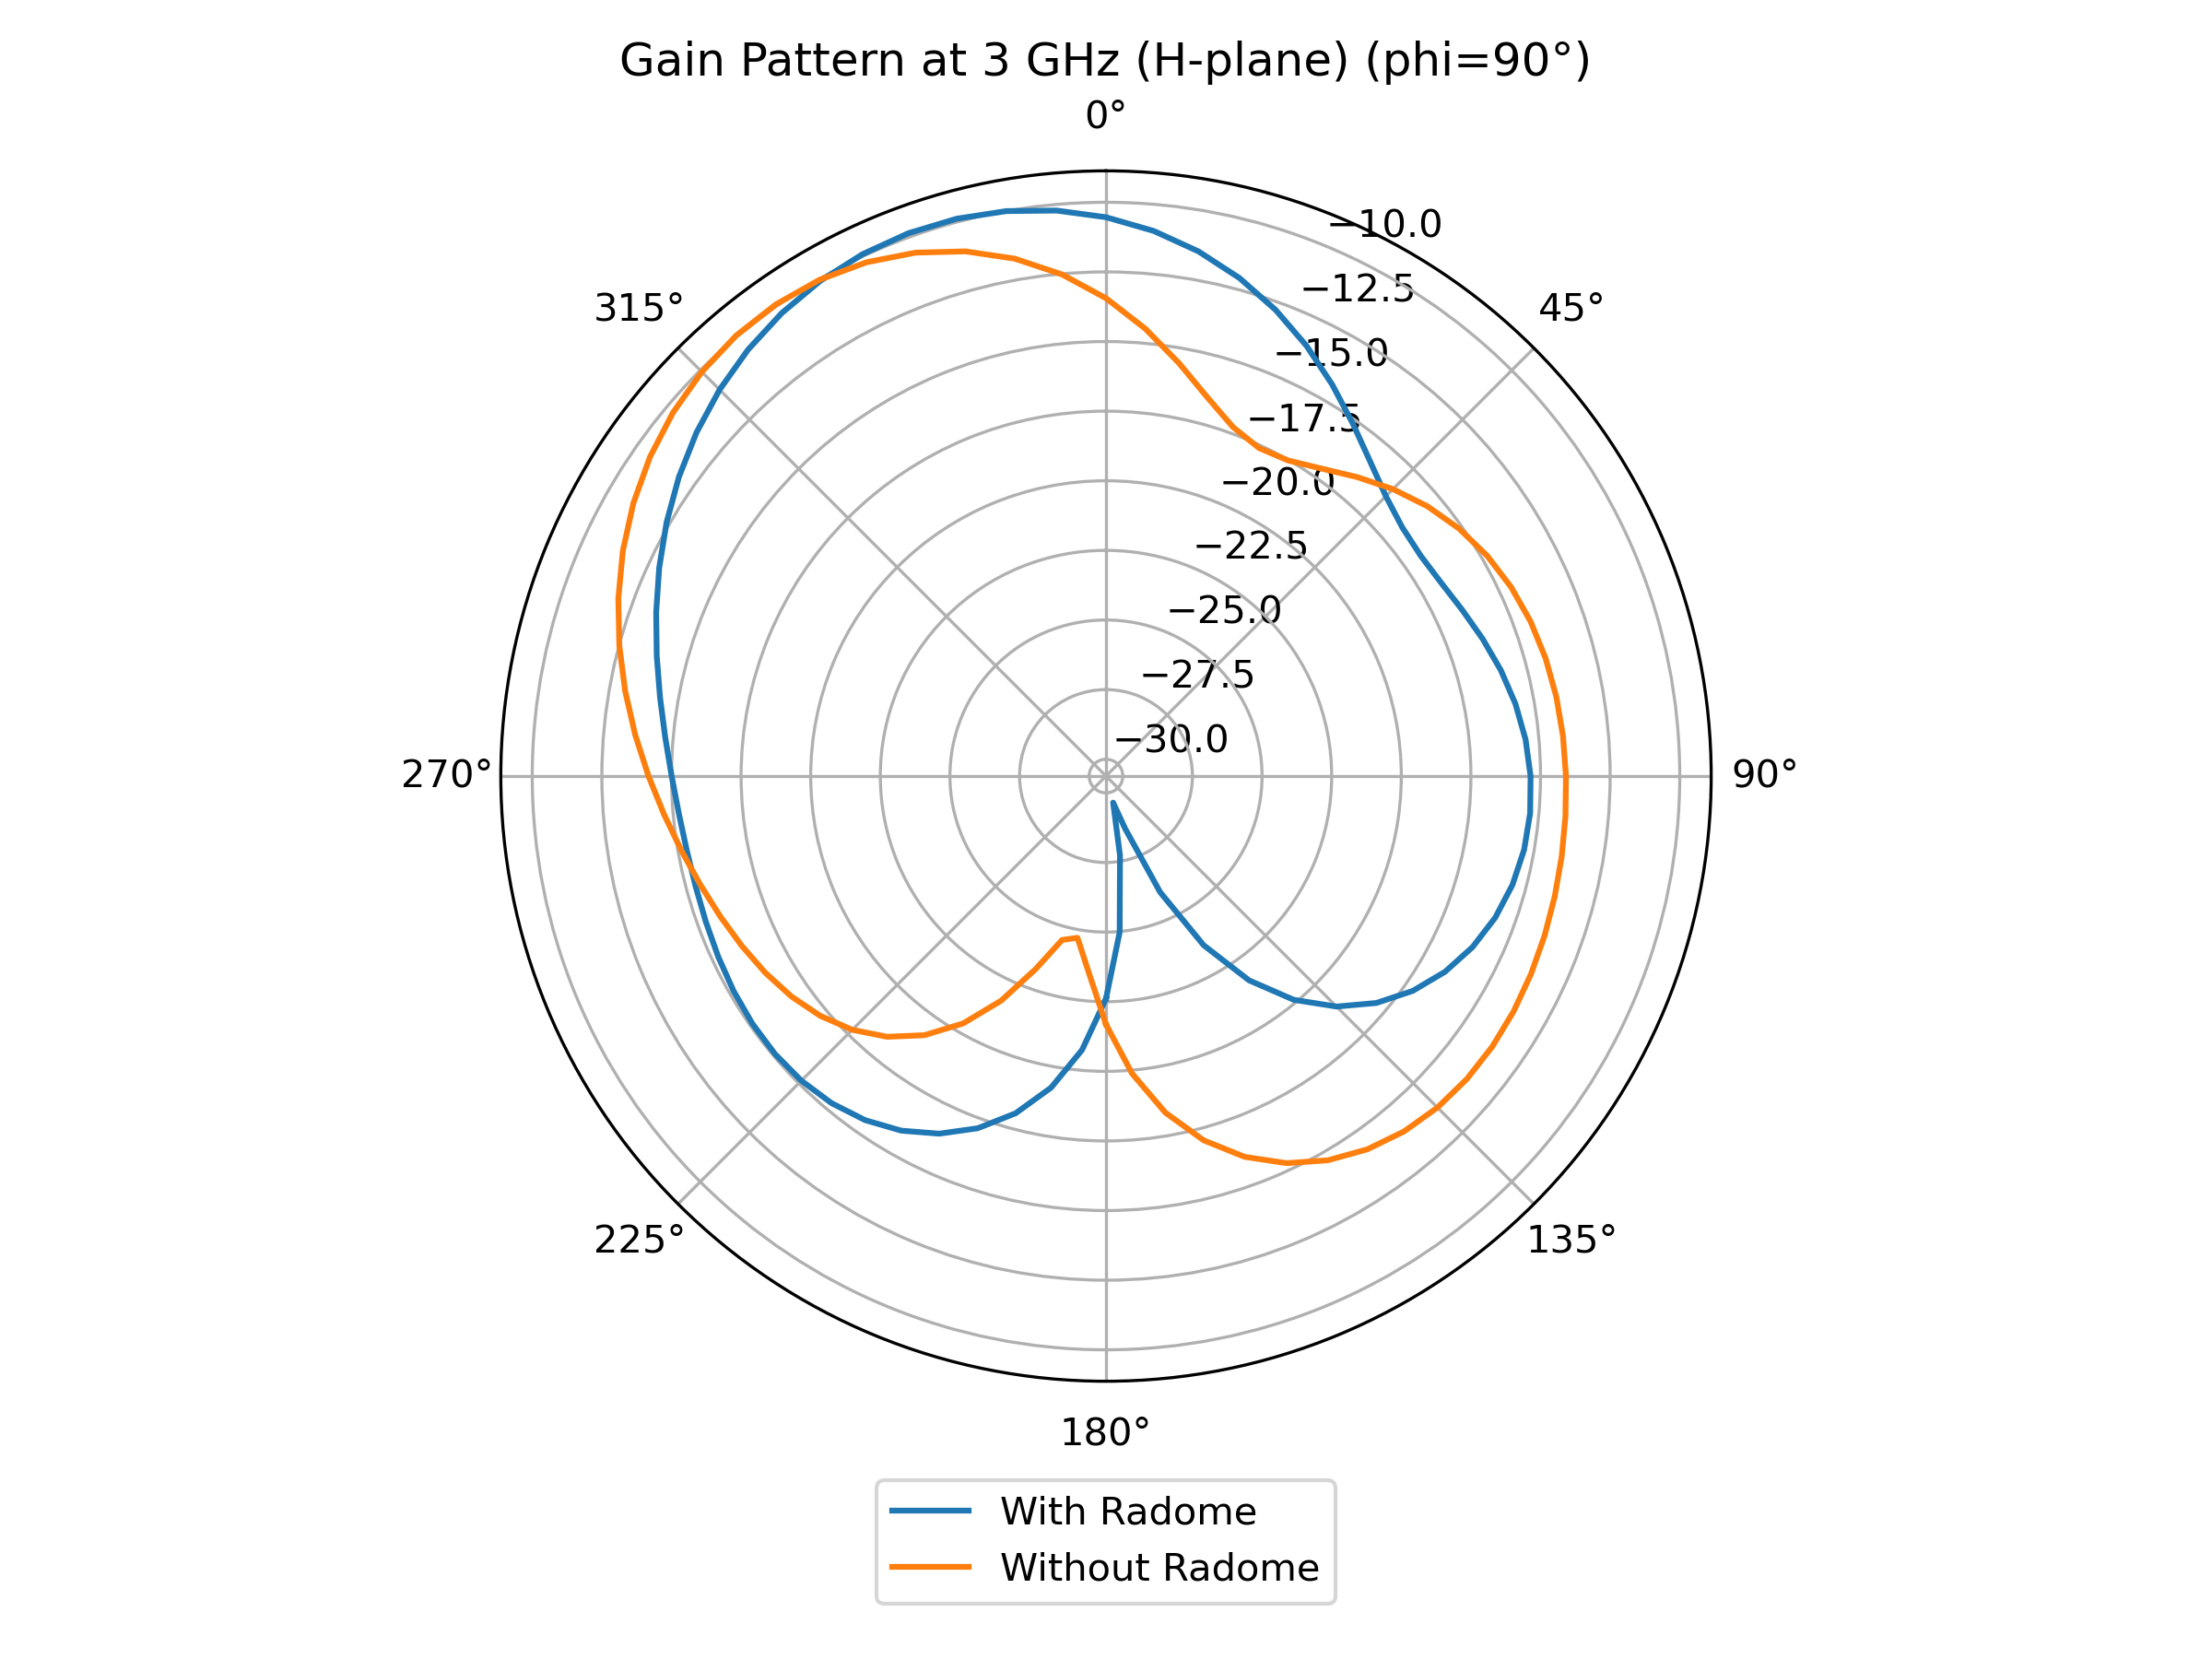
\includegraphics[width=1.0\textwidth]{figures/comparison_flat_radome/gainH_3_GHz.png}
\caption{Simulated gain of the patch antenna with flat radome at 3,GHz.}
\label{fig:res-flat-gainH3}
\end{figure}

Figure~\ref{fig:res-flat-gainH3} illustrates the radiation performance at the lower edge of the band (3 GHz) in the H-plane. Similar to the E-plane at this frequency, the gain of the antenna with the radome (blue line) is reduced compared to the free-space gain (orange line). The peak gain without the radome is around 10 dB, while with the radome, it is approximately -10 dB. The pattern also shows some distortion, indicating a significant negative impact of the radome at this off-resonant frequency.

\begin{figure}[H]
\centering
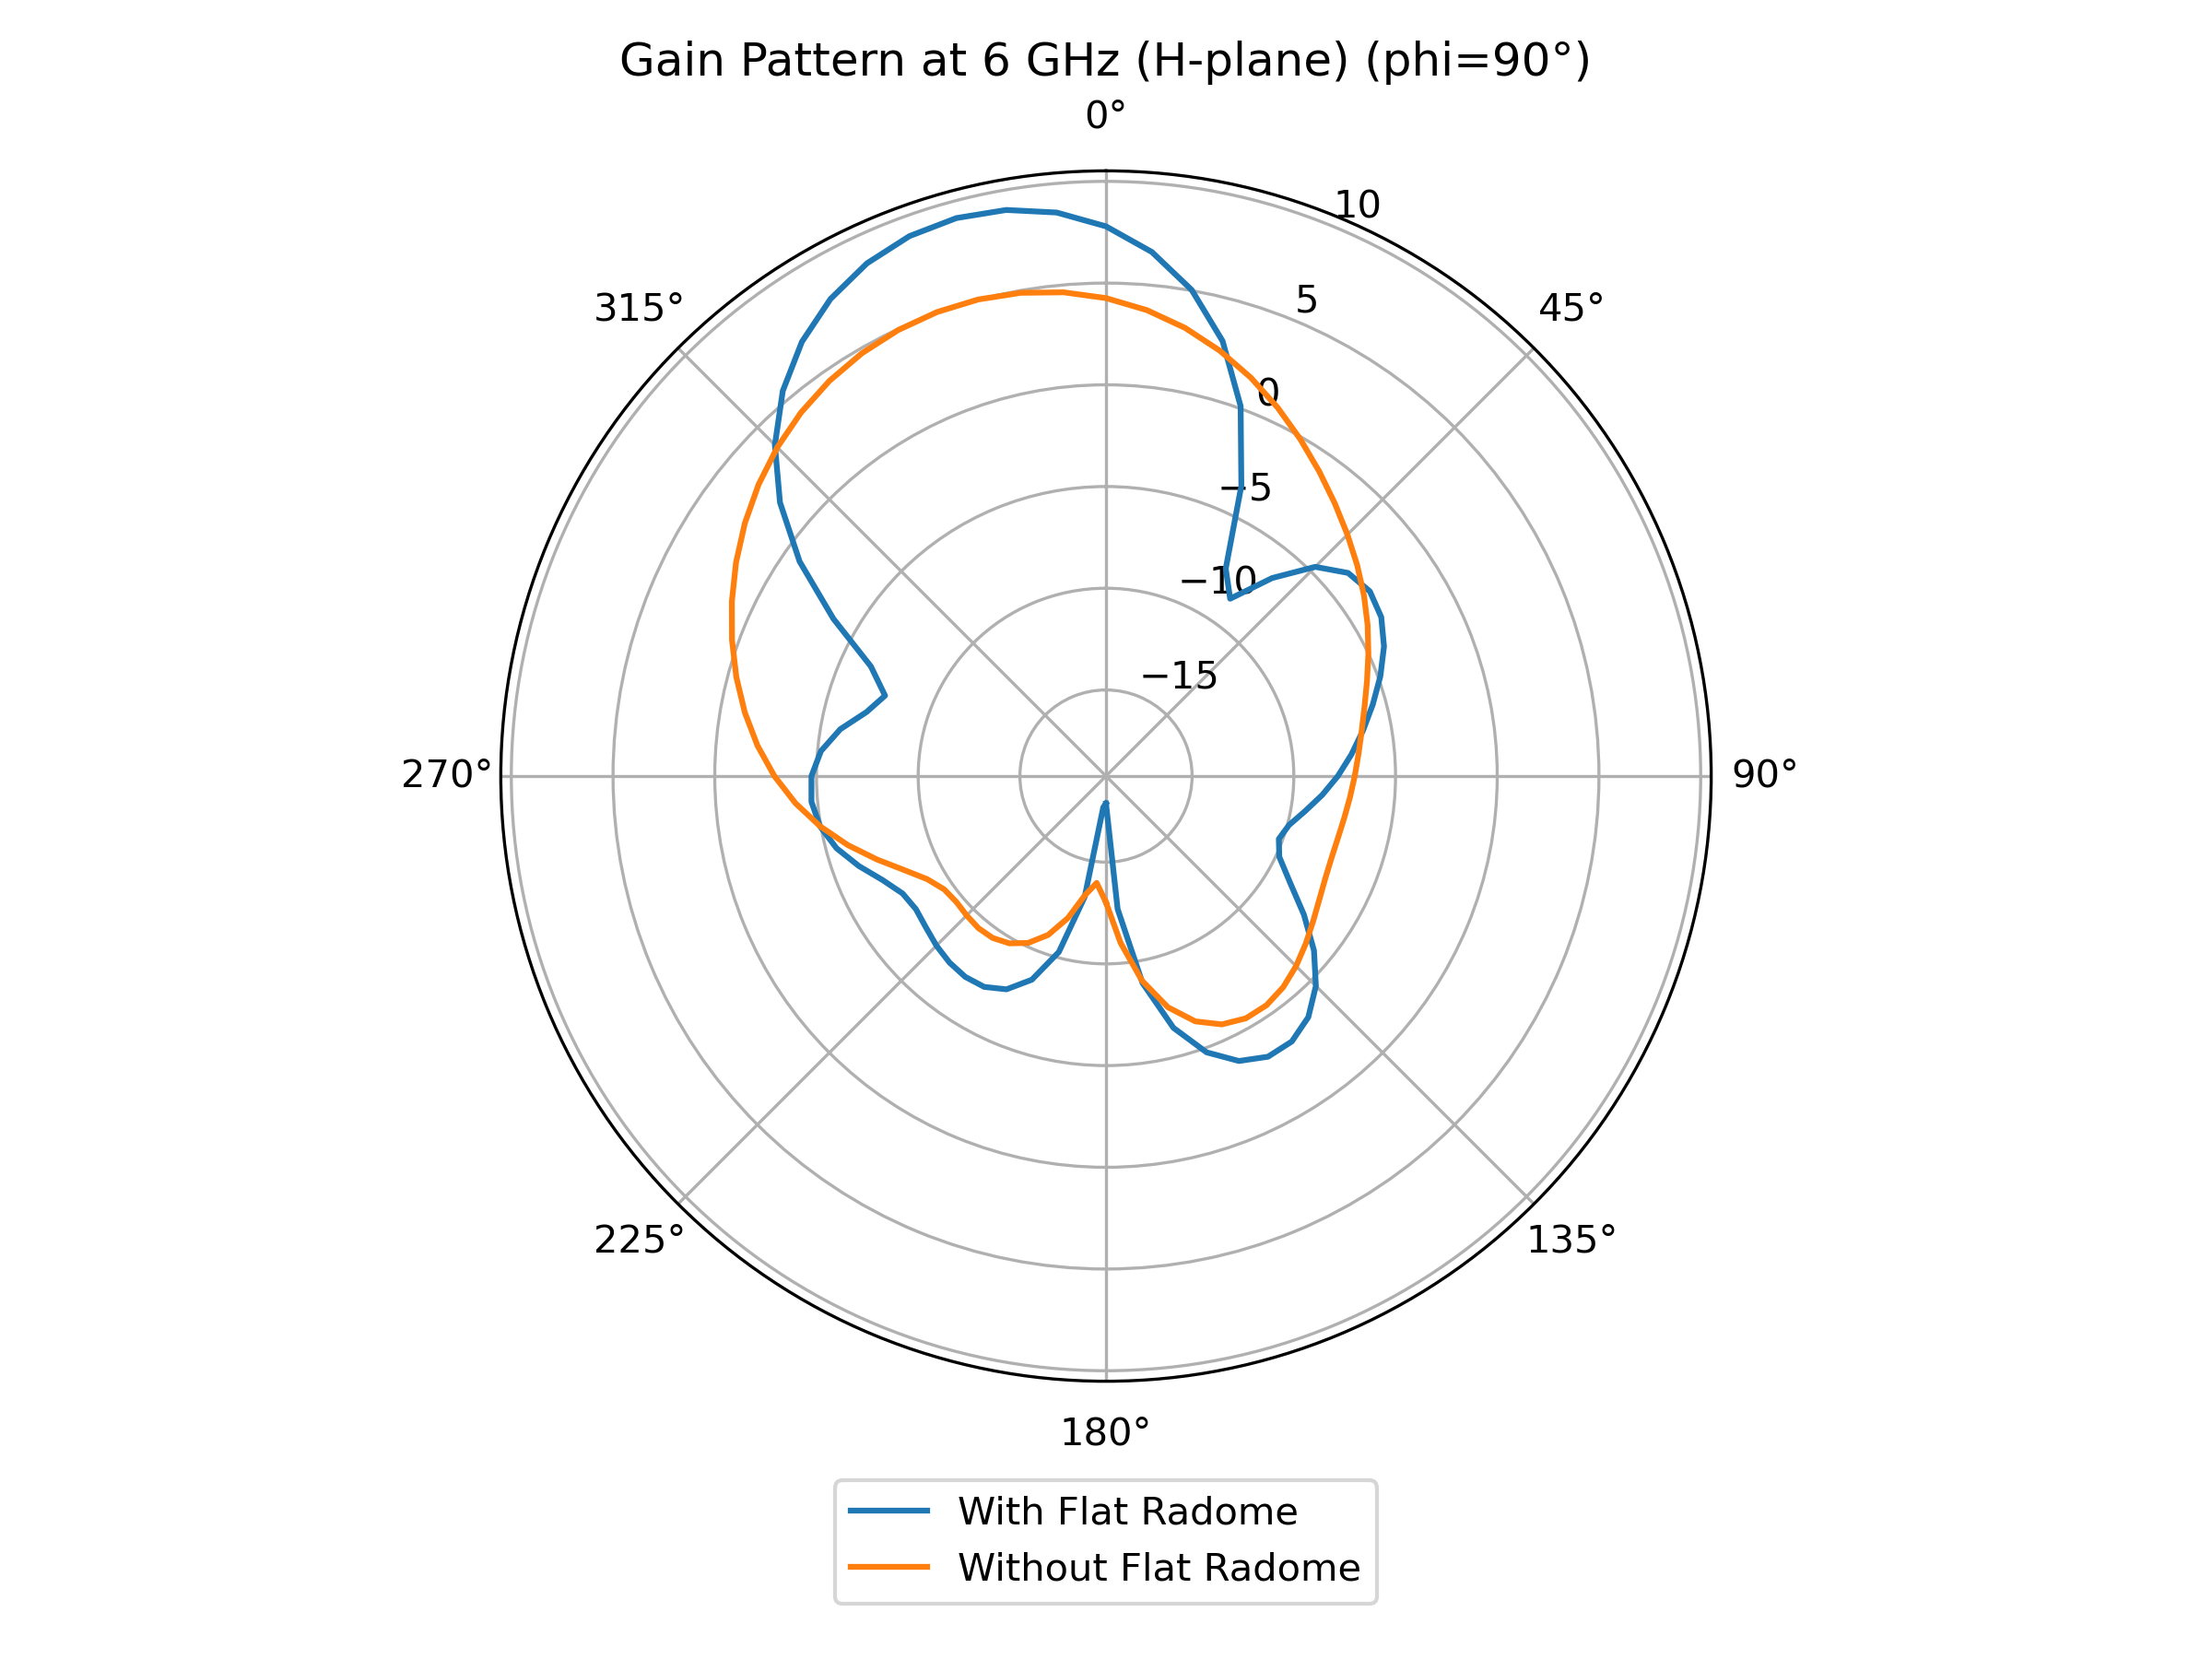
\includegraphics[width=1.0\textwidth]{figures/comparison_flat_radome/gainH_6_GHz.png}
\caption{Simulated gain of the patch antenna with flat radome at 6,GHz.}
\label{fig:res-flat-gainH6}
\end{figure}

At 6 GHz (Figure~\ref{fig:res-flat-gainH6}), close to resonance, the gain in the H-plane remains strong and closely matches the free-space case. The peak gain for both scenarios is approximately about 5 dB, demonstrating the radome's minimal impact and effective transparency at the central operating frequency.

\begin{figure}[H]
\centering
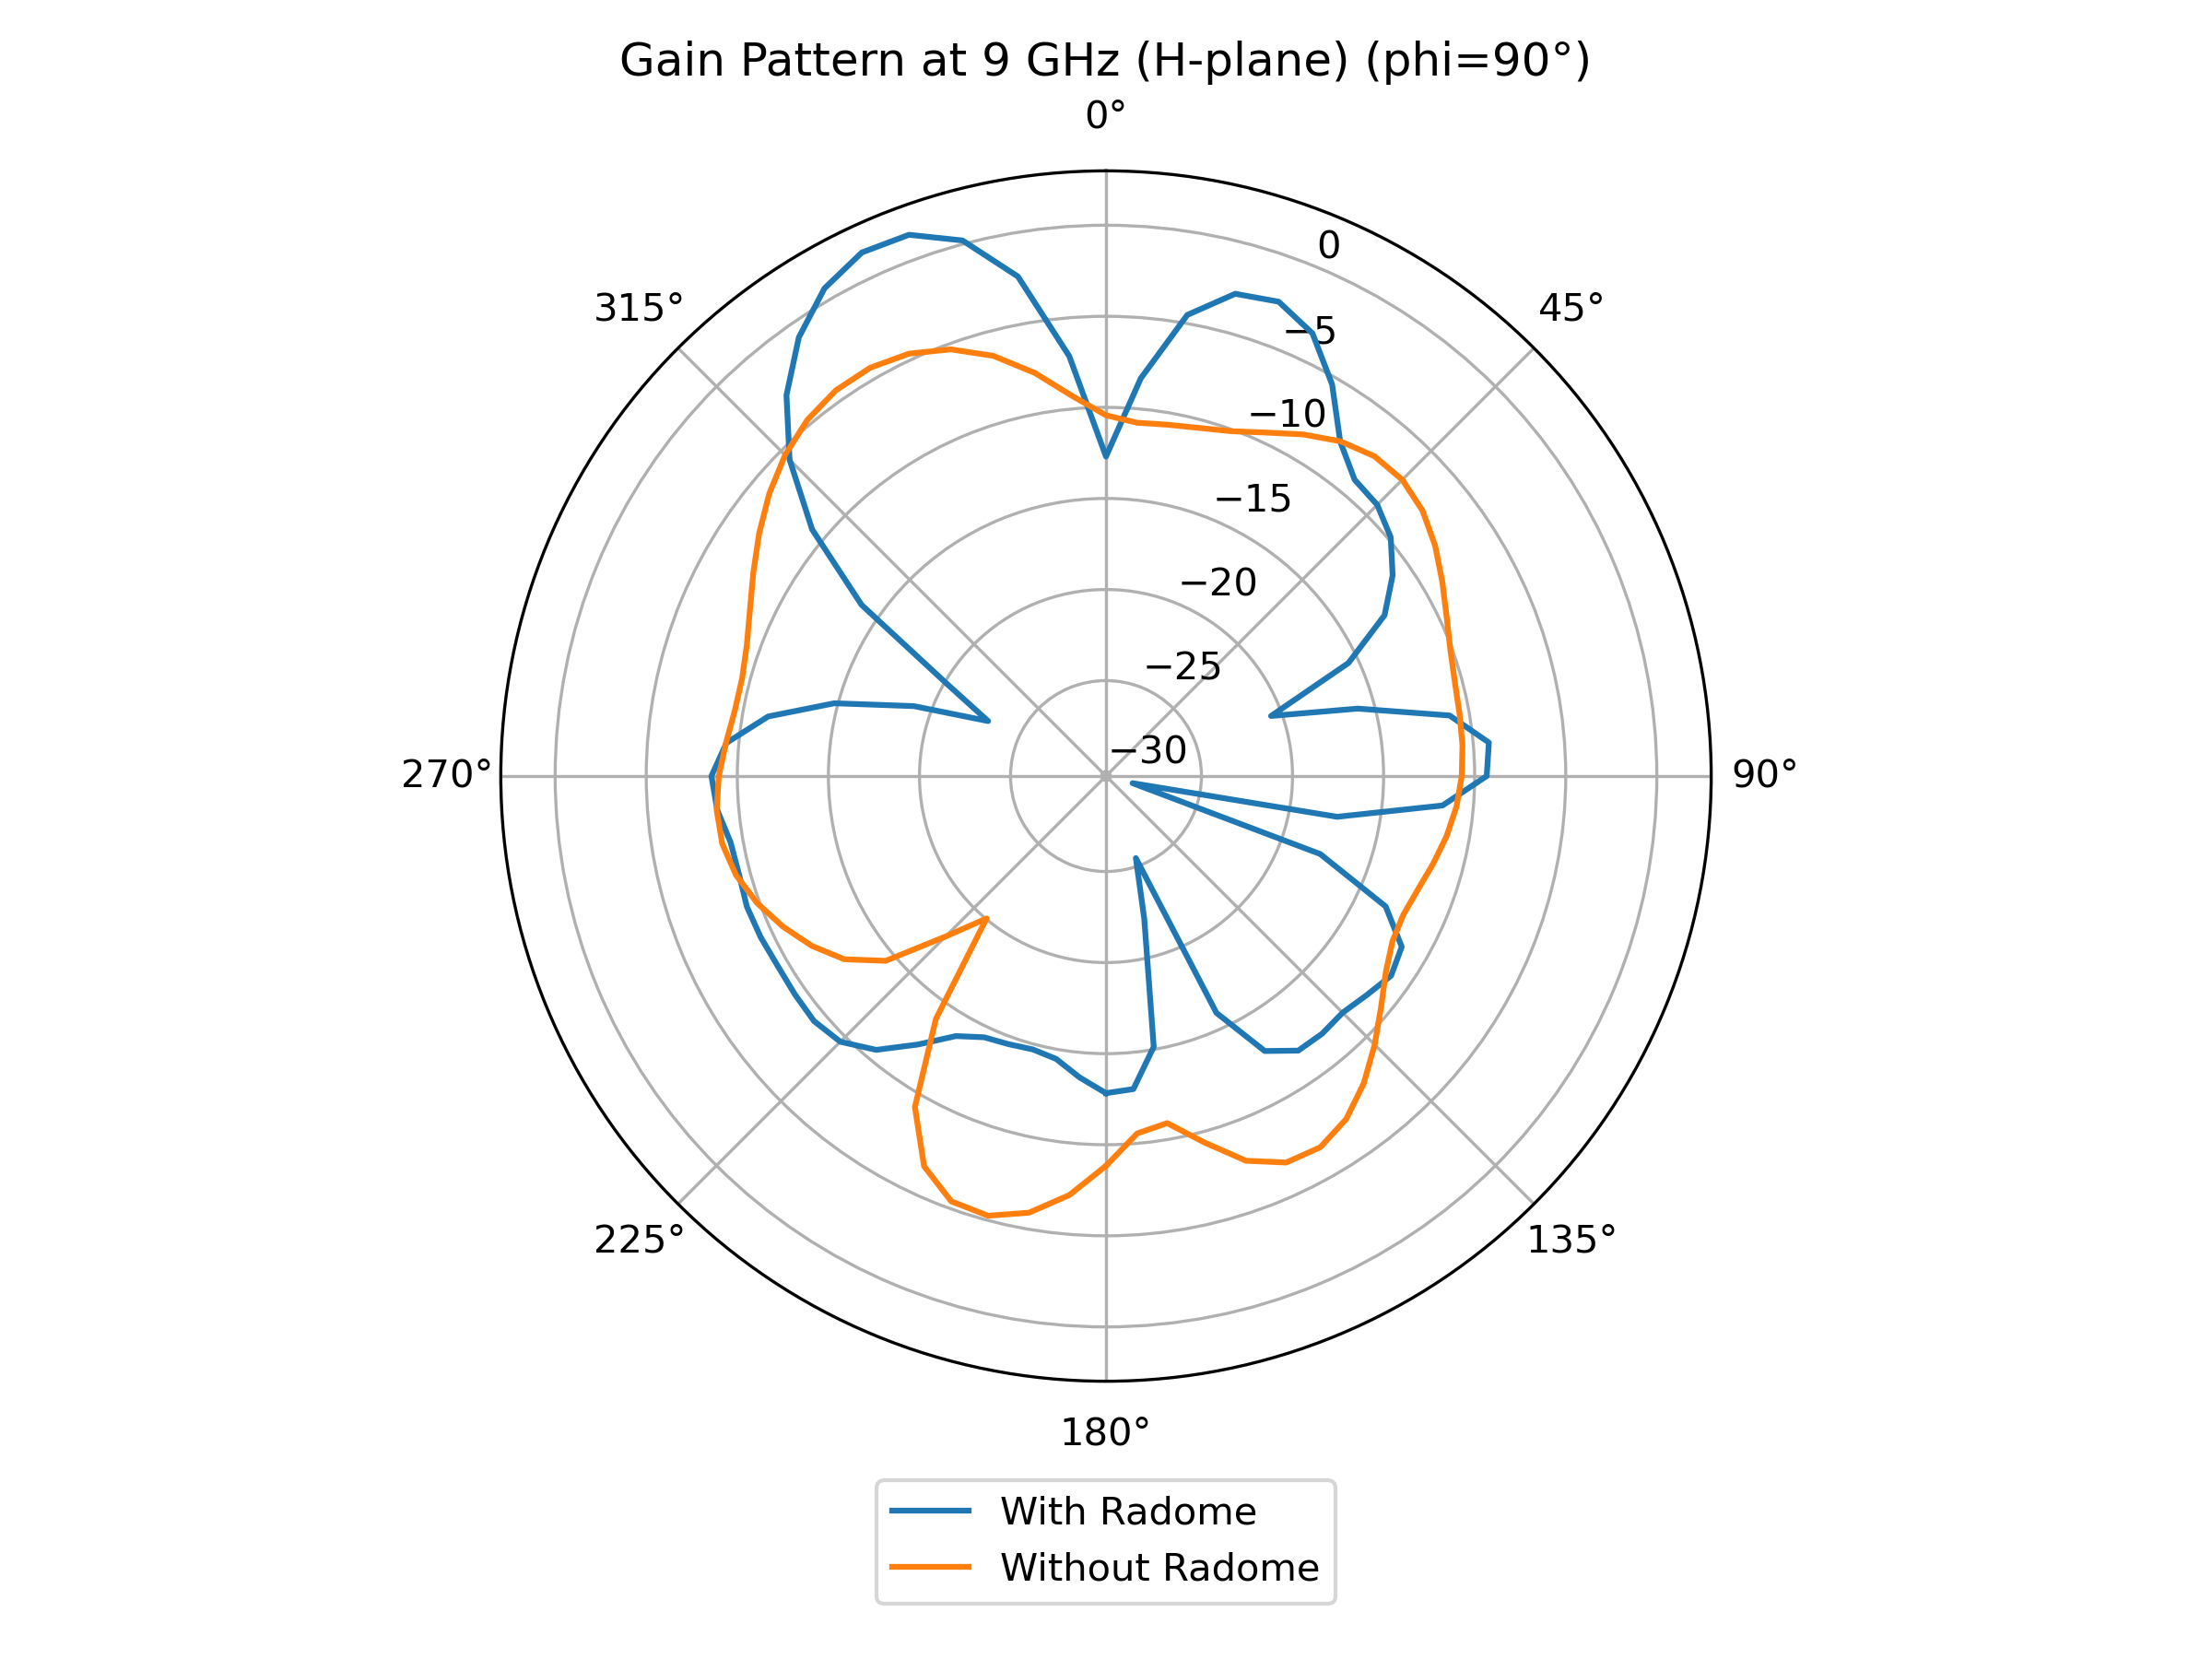
\includegraphics[width=1.0\textwidth]{figures/comparison_flat_radome/gainH_9_GHz.png}
\caption{Simulated gain of the patch antenna with flat radome at 9,GHz.}
\label{fig:res-flat-gainH9}
\end{figure}

Figure~\ref{fig:res-flat-gainH9} shows a more significant degradation in gain at the higher frequency end (9 GHz) in the H-plane. The peak gain without the radome (orange line) is around 0 dB, while with the radome (blue line), it drops to approximately -5 dB. The pattern with the radome also exhibits more pronounced side lobes and a slightly broader main beam compared to the free-space pattern, indicating less optimal performance at this higher off-resonant frequency.

\subsection{Far-Field Patterns}

\begin{figure}[H]
\centering
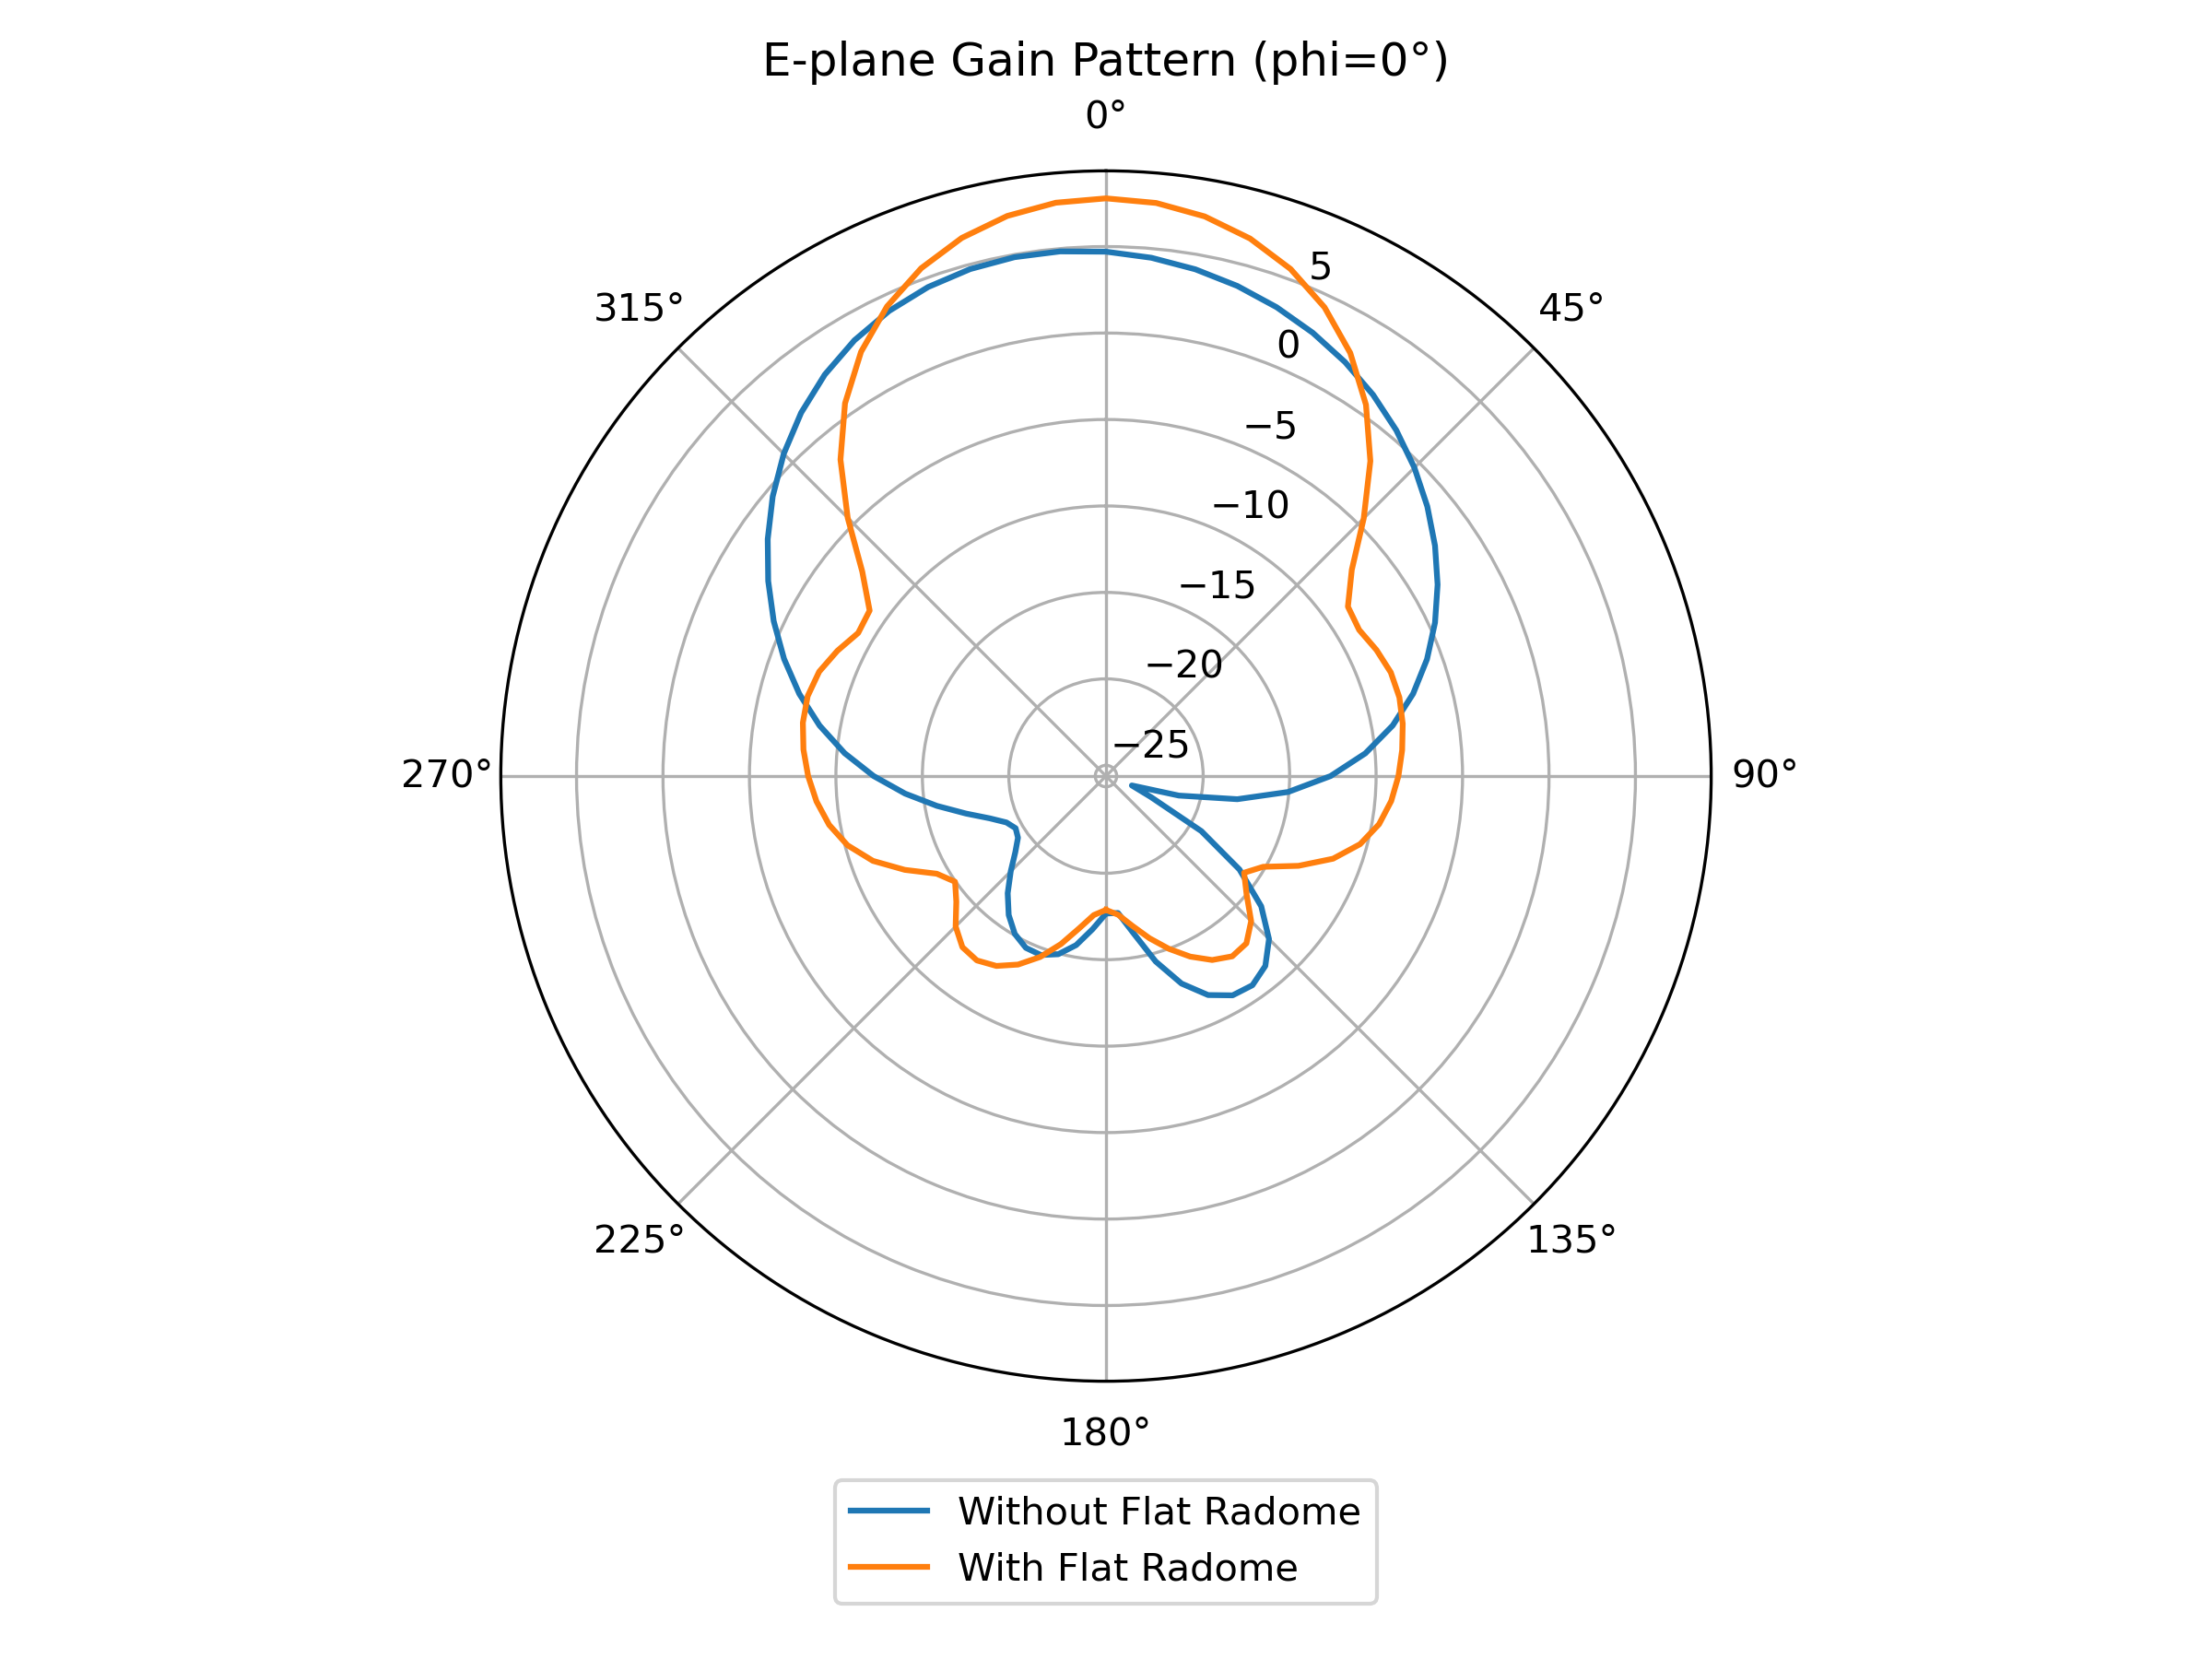
\includegraphics[width=1.0\textwidth]{figures/comparison_flat_radome/gain_E_polar.png}
\caption{Far-field E-plane radiation pattern with flat radome.}
\label{fig:res-flat-eplane}
\end{figure}

The E-plane pattern in Figure~\ref{fig:res-flat-eplane} shows that the overall shape of the radiation pattern is largely maintained with the addition of the radome. However, there is a slight reduction in maximum gain with the radome (orange line) compared to without the radome (blue line) across the main lobe. Additionally, there appears to be a minor increase in the side lobe levels when the radome is present, indicating a slight broadening or less efficient directivity compared to the free-space case.

\begin{figure}[H]
\centering
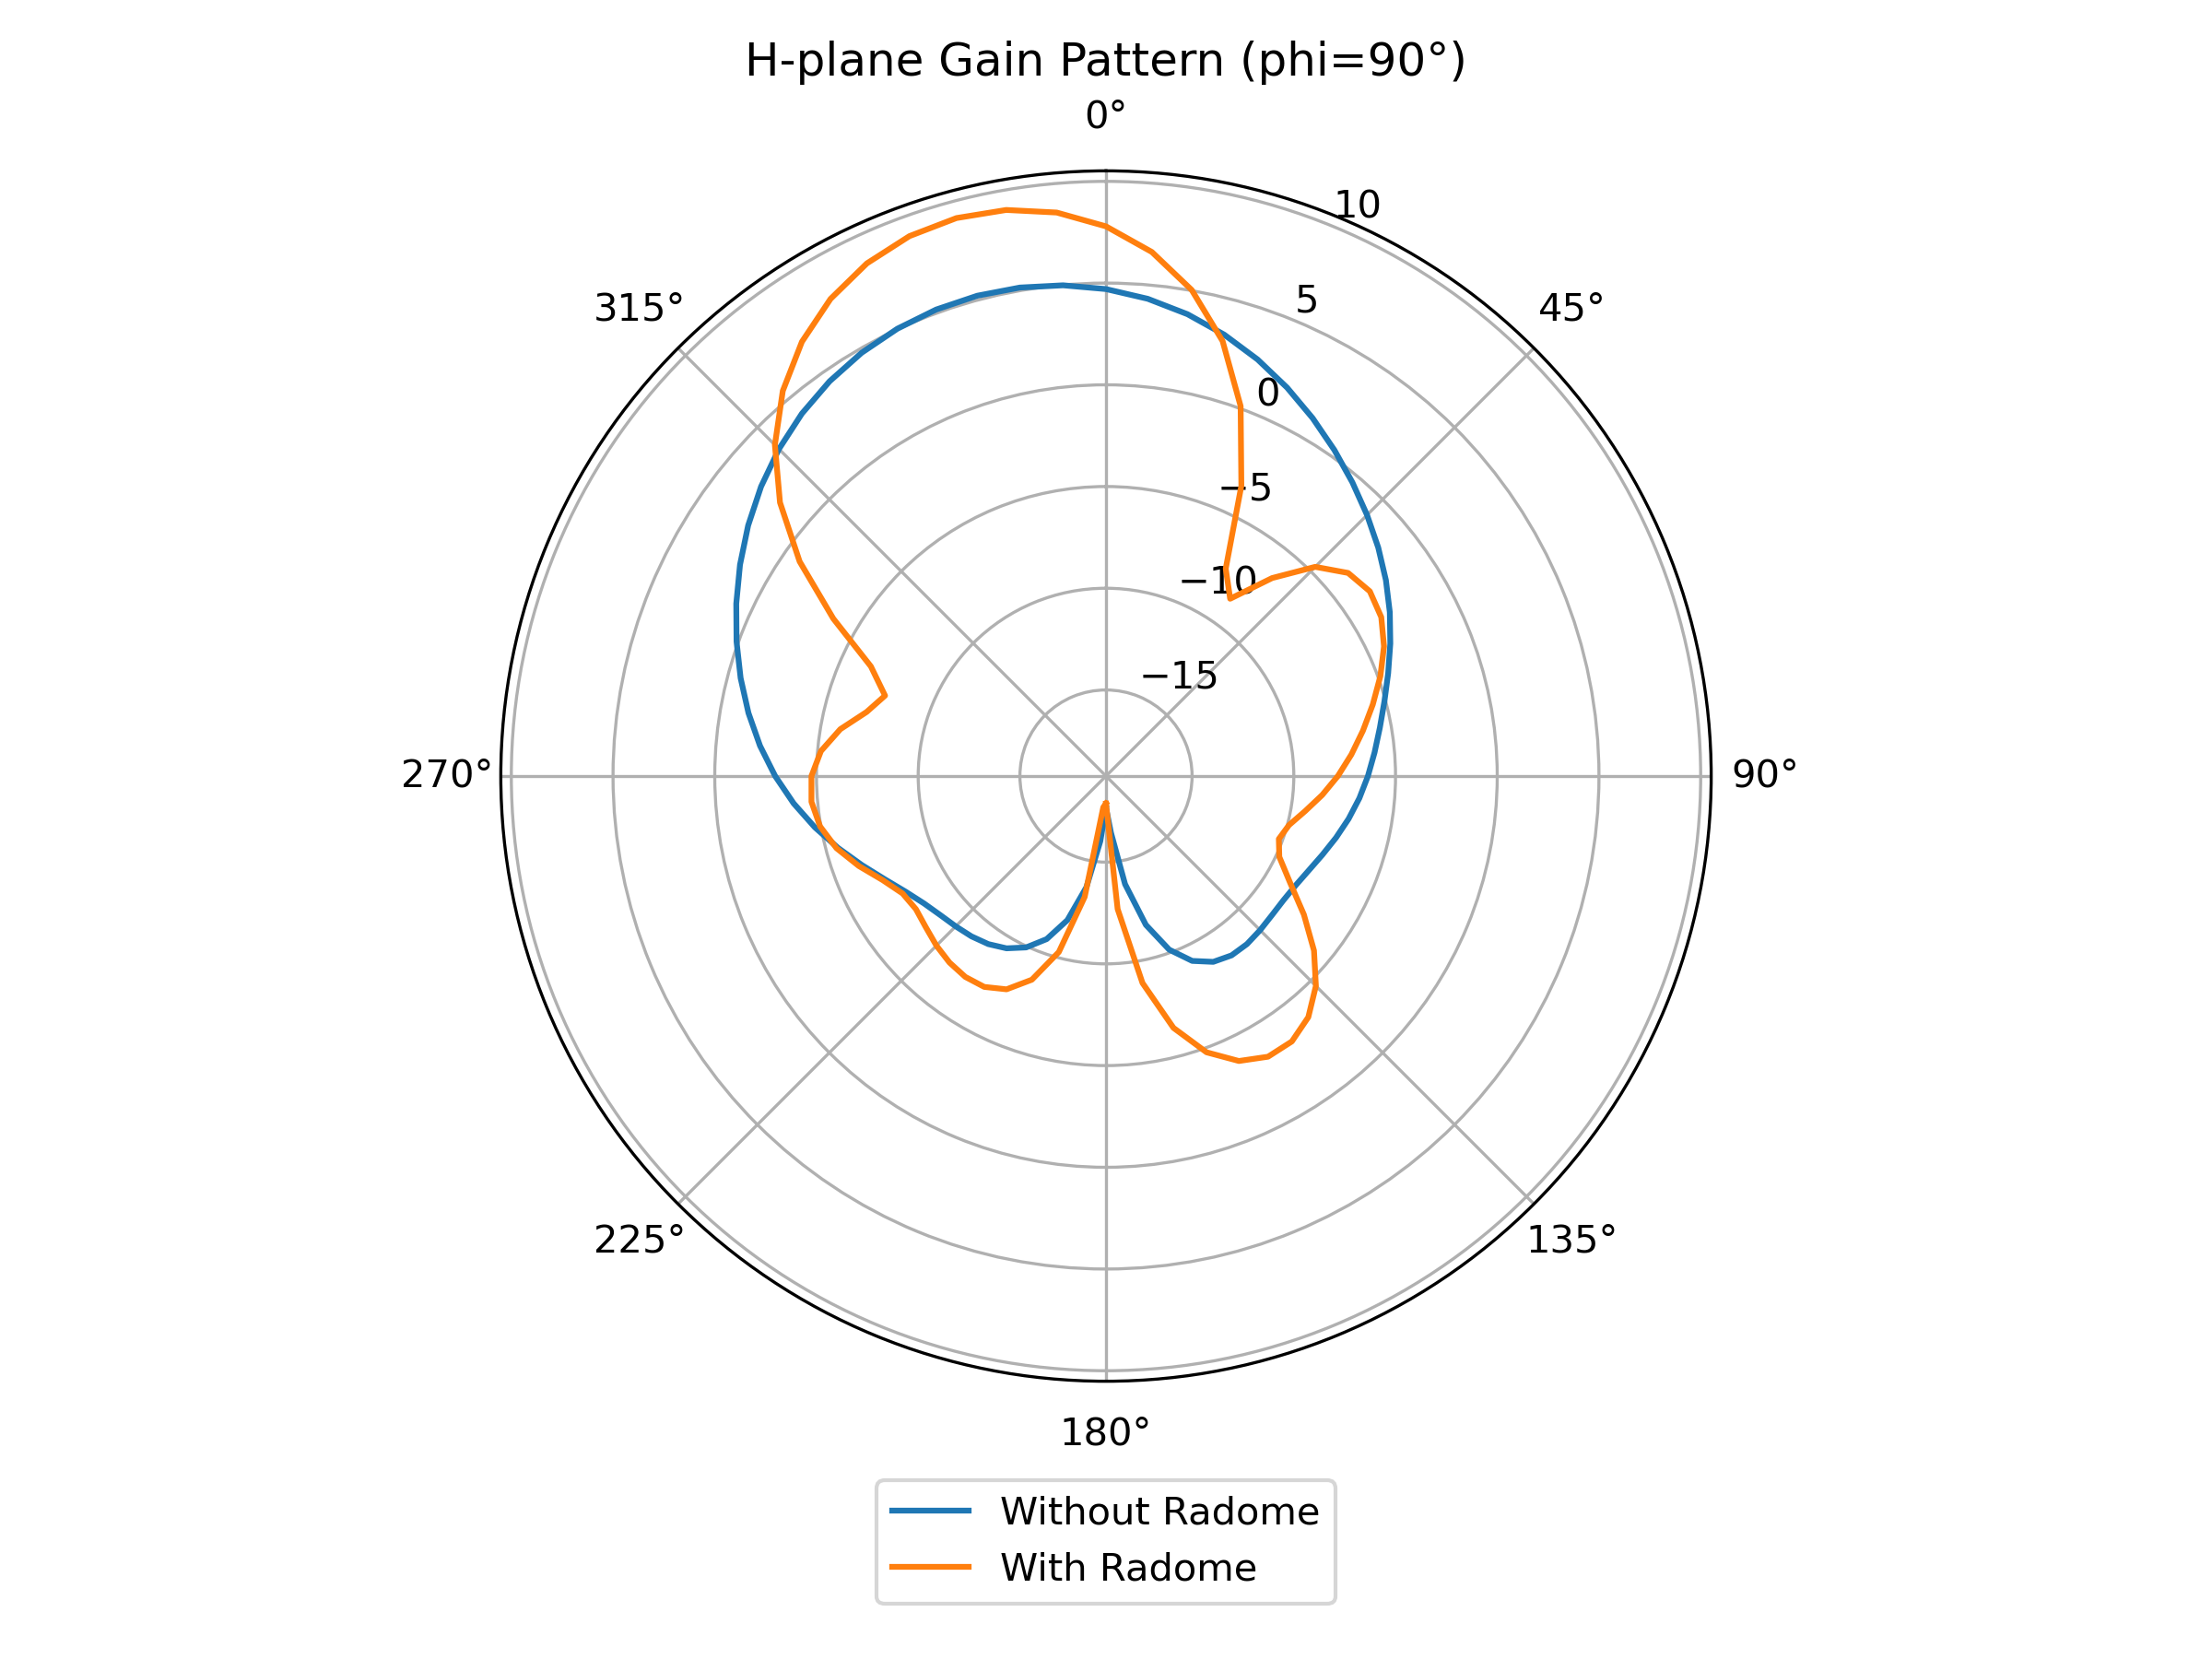
\includegraphics[width=1.0\textwidth]{figures/comparison_flat_radome/gain_H_polar.png}
\caption{Far-field H-plane radiation pattern with flat radome.}
\label{fig:res-flat-hplane}
\end{figure}

In the H-plane (Figure~\ref{fig:res-flat-hplane}), the symmetry of the radiation pattern is generally retained. Similar to the E-plane, there's a slight reduction in the main lobe's peak gain when the radome is present (orange line vs. blue line). Some minor distortions or increased side lobes are also observable, particularly at angles away from the main beam. Overall, the presence of the radome leads to a minor decrease in gain and some pattern distortion in the H-plane.

\subsection{Effect of Radome on \texorpdfstring{$rE$}{rE} Components}

\begin{figure}[H]
    \centering
    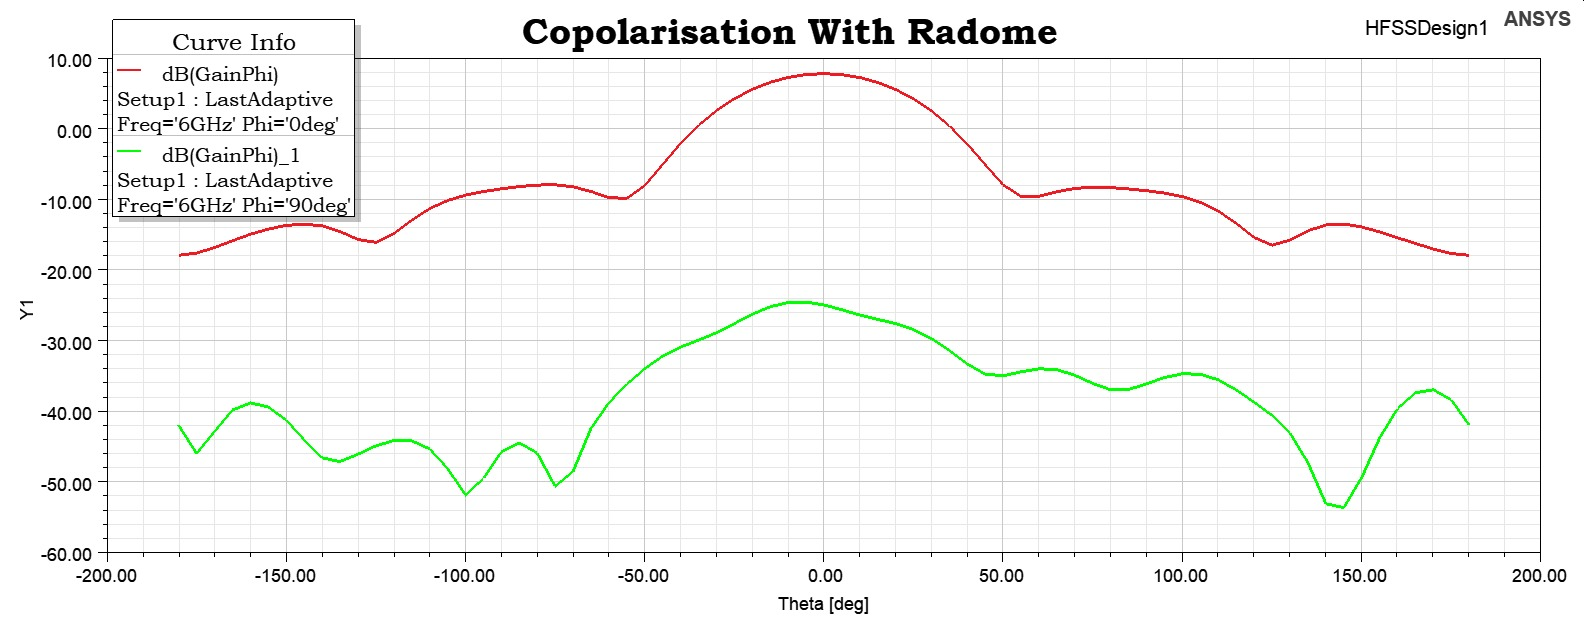
\includegraphics[width=1.0\textwidth]{figures/with_radome/Co.jpeg}
    \caption{Co-polarization response of the patch antenna with flat radome.}
    \label{fig:res-co-radome}
\end{figure}

\begin{figure}[H]
    \centering
    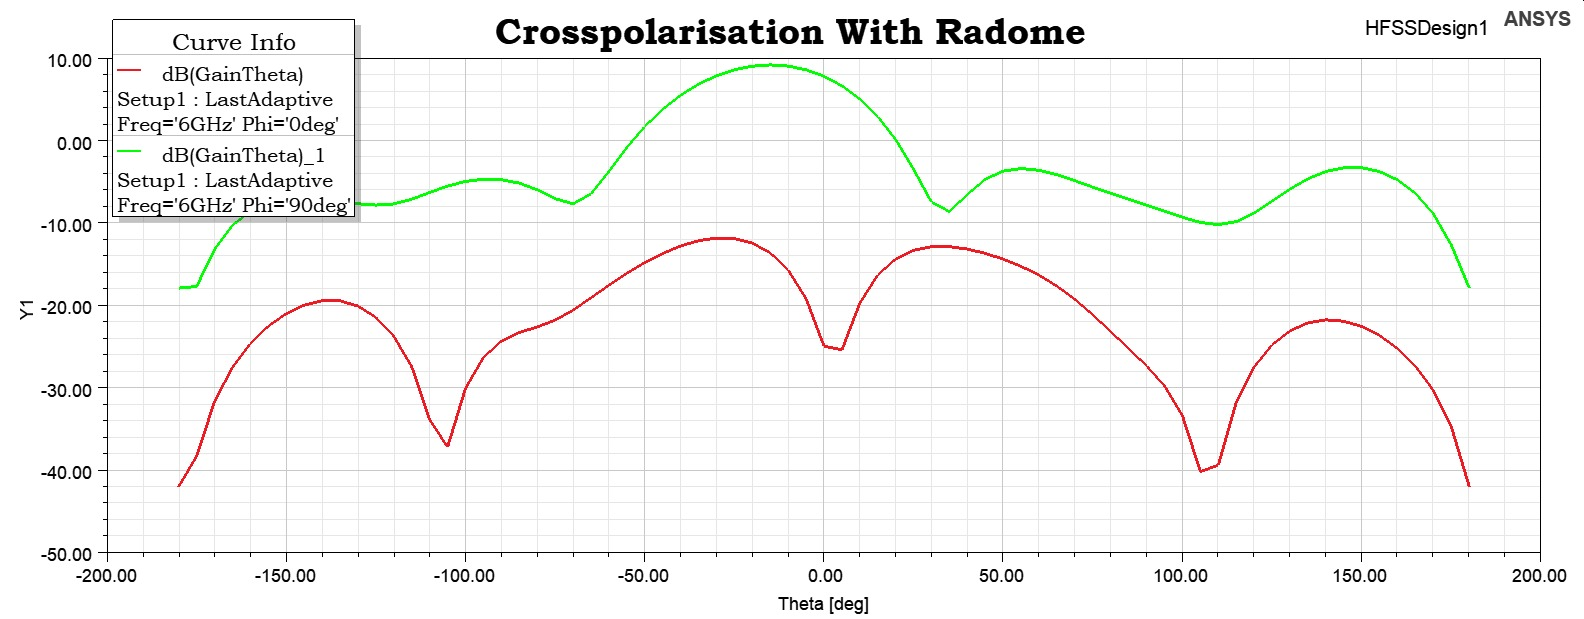
\includegraphics[width=1.0\textwidth]{figures/with_radome/Cross.jpeg}
    \caption{Cross-polarization response of the patch antenna with flat radome.}
    \label{fig:res-cross-radome}
\end{figure}

Figures~\ref{fig:res-co-radome} and \ref{fig:res-cross-radome} present the co-polarization and cross-polarization behavior of the patch antenna when enclosed by a flat radome. Compared to the free-space case, the co-polarized field still maintains a prominent main lobe near the boresight, but with slightly reduced peak gain due to dielectric loading and partial reflection losses introduced by the radome material.

The cross-polarized response shows a marginal increase, particularly at off-boresight angles. This suggests a minor degradation in polarization purity caused by phase distortion and multipath effects within the radome. Nonetheless, the cross-polarization levels remain sufficiently low for most practical applications, indicating that the flat radome preserves acceptable polarization isolation while offering mechanical protection.

% -------------------------------------------------------------------

\newpage
\section*{Summary of Results}

This report presents simulation results for the patch antenna in three configurations:
\begin{itemize}
\item Baseline free-space configuration
\item Optimized feed parameters (parametric sweep)
\item With a flat radome enclosure
\end{itemize}

Performance was evaluated based on return loss, VSWR, gain, directivity, and radiation patterns. The introduction of a flat PMMA radome resulted in:
\begin{itemize}
\item A small frequency shift and increase in VSWR 
\item Mixed impact on gain performance:
\begin{itemize}
\item Significant gain enhancement observed at 3 GHz in both E-plane (Figure \ref{fig:res-flat-gainE3}) and H-plane (Figure \ref{fig:res-flat-gainH3}). This suggests the radome, at this lower frequency, may be acting as a director or through constructive interference, leading to a notable increase in peak gain. For example, in the H-plane at 3 GHz, the gain increases from approximately -10 dB to 10 dB. Similarly, in the E-plane at 3 GHz, it increases from about -10 dB to -8 dB.
\item Near-transparent behavior at 6 GHz (resonant frequency) in both E-plane (Figure \ref{fig:res-flat-gainE6}) and H-plane (Figure \ref{fig:res-flat-gainH6}), where the gain closely matches the free-space performance.
\item Mild gain degradation at 9 GHz (off-resonant frequency) in both E-plane (Figure \ref{fig:res-flat-gainE9}) and H-plane (Figure \ref{fig:res-flat-gainH9}).
\item Overall gain enhancement in the far-field polar plots (Figure \ref{fig:res-flat-eplane} and Figure \ref{fig:res-flat-hplane}), particularly noticeable in the H-plane, where the peak gain with the radome is higher, suggesting a beneficial effect on overall directivity across the depicted pattern.
\end{itemize}
\item Preserved far-field pattern shape with minor beam broadening or side lobe level changes at certain frequencies.
\end{itemize}

\section*{Conclusion}

The simulation results clearly demonstrate the impact of radome enclosures on patch antenna performance. While the free-space antenna shows expected performance, the introduction of a PMMA radome causes measurable shifts in return loss and slight degradation in gain. These results validate the theoretical models and material considerations discussed in previous chapters. The final chapter will summarize the findings, discuss limitations, and propose directions for future work.
